%% ICML submission. Provisional format: the ICML 2026 kit (paper/style/icml2026), to be
%% swapped for the 2027 kit when released -- change the three symlinks in paper/ and the
%% \usepackage line below; nothing else in this file depends on the kit version.
%% Page geometry, fonts and spacing are the kit's; they are never altered here.
\documentclass{article}

\usepackage{microtype}
\usepackage{graphicx}
\usepackage{booktabs}
\usepackage{array}
\usepackage{multirow}
\usepackage{xcolor}
\usepackage{hyperref}
\usepackage{tikz}
\usetikzlibrary{calc,arrows.meta,positioning}
\newcommand{\theHalgorithm}{\arabic{algorithm}}

% Submission: anonymous. Camera-ready: \usepackage[accepted]{icml2026}.
\usepackage{icml2026}

\usepackage{amsmath}
\usepackage{amssymb}
\usepackage{mathtools}
\usepackage{amsthm}
\usepackage[capitalize,noabbrev]{cleveref}

\theoremstyle{plain}
\newtheorem{theorem}{Theorem}
\newtheorem{proposition}[theorem]{Proposition}
\newtheorem{lemma}[theorem]{Lemma}
\newtheorem{corollary}[theorem]{Corollary}
\theoremstyle{definition}
\newtheorem{assumption}[theorem]{Assumption}
\theoremstyle{remark}
\newtheorem{remark}[theorem]{Remark}

\graphicspath{{figures/}}
% ===========================================================================
% Shared notation for the internal note and the compendium.
%
% Conventions follow the statistical-physics usage of the diffusion literature
% (Song et al. 2021 for the SDE formulation; Mezard-Montanari 2009 for the
% graphical-model side). Only publicly available sources are cited.
% docs/NOTATION.md is the reference for every symbol below, for the code names
% that carry them, for the collaborators' note, and for the thesis concordance.
%
% Symbol decisions that matter, fixed here once:
%
%   1. K (or K_theta) is the MARKOV TRANSITION KERNEL, everywhere and only.
%      The number of quadrature grid points is N_g. These were previously W and
%      K respectively, which collided; nothing in either document may now use
%      K for a grid size or W for a kernel. The phi^4 transfer operator
%      e^{-W} is \transfer (sans-serif T), never K.
%
%   2. The chain length is L, and every graphical-model statement is indexed by
%      sites. The ambient dimension equals it, n = L, but the two are written
%      separately because they are different concepts and the reader should not
%      have to infer the identification. The number of observed sequences is M,
%      and never the grid size.
%      A translation sentence appears at first use, because much of the
%      diffusion literature uses n for the sample count and d for the dimension.
%
%   3. The decay factor is written e^{-t} in displayed equations. Where a proof
%      abbreviates it, the abbreviation is alpha = e^{-t}, declared, never
%      alpha_t and never anything else (the code's argument `alpha` is the same
%      object).
%
%   4. Gaussian white noise eta is STANDARDISED, <eta(t)eta(t')> = delta(t-t'),
%      so the sqrt(2) is carried explicitly in both the forward and the reverse
%      SDE. This keeps Delta_t = 1 - e^{-2t} consistent throughout.
%
%   5. Vectors are bold lowercase (\vect) and matrices and tensors are bold
%      uppercase (\mat). Scalars, including single sites a_i, stay upright.
%      Anything indexed down to a scalar loses its bold.
%
%   6. BP messages are the cavity messages \lmsg_i, \rmsg_i: both EXCLUDE the
%      local likelihood ell_i, and the site marginal is \lmsg_i ell_i \rmsg_i.
%      (The collaborators' note writes alpha_i = \lmsg_i ell_i and beta_i =
%      \rmsg_i.) Posterior marginals are written out, p(a_i | x), because gamma
%      and xi are taken (6 and 7 below).
%
%   7. The chain's driving noise is eps_i with density p_eps and variance q; the
%      word "innovation" is not used (the 25 Sep call). The linear chain with
%      Laplace driving noise, not "the Laplace AR(1)".
%
%   8. Greek letters with one meaning each: gamma the phi^4 bond variance
%      (the Gaussian reference measure is \gref); xi the correlation length;
%      beta the generalised-Gaussian exponent; delta a misspecification
%      strength; h the lattice spacing (the quadrature spacing is \gridh).
% ===========================================================================

% --- Diffusion -------------------------------------------------------------
\newcommand{\Pz}{P_0}                       % clean distribution
\newcommand{\Pt}{P_t}                       % noised distribution at time t
\newcommand{\Dt}{\Delta_t}                  % 1 - e^{-2t}
\newcommand{\score}{S}                      % S(x,t) = grad log P_t(x)
\newcommand{\gwn}{\vect{\eta}}              % standardised Gaussian white noise (vector)
\newcommand{\tmin}{t_{\min}}
\newcommand{\tmax}{t_{\max}}

% Posterior mean, in bracket notation rather than E[a|x].
\newcommand{\pmean}[1]{\langle #1 \rangle_{x,t}}
\newcommand{\pmeansite}[1]{\langle a_{#1} \rangle_{x,t}}

% --- Vectors and matrices --------------------------------------------------
% Bold lowercase for vectors, bold uppercase for matrices and tensors.
\newcommand{\vect}[1]{\mathbf{#1}}
\newcommand{\mat}[1]{\mathbf{#1}}
\newcommand{\va}{\vect{a}}                  % clean chain, in R^L
\newcommand{\vx}{\vect{x}}                  % noised chain, in R^L
\newcommand{\vz}{\vect{z}}                  % standard normal draw, in R^L
\newcommand{\Sig}{\mat{\Sigma}}             % covariance
\newcommand{\Id}{\mat{I}}                   % identity

% --- Chain and graphical model --------------------------------------------
\newcommand{\nsites}{L}                     % chain length (ambient dimension n = L)
\newcommand{\nseq}{M}                       % number of observed sequences
\newcommand{\ngrid}{N_{\mathrm{g}}}         % number of quadrature grid points
\newcommand{\gridpt}[1]{u_{#1}}             % grid point
\newcommand{\gridh}{\Delta u}                % quadrature grid spacing (h is the lattice spacing)
\newcommand{\halfwidth}{A}                  % grid half-width, domain [-A, A]
\newcommand{\kernel}{K}                     % transition kernel K(a'|a)
\newcommand{\kernelth}{K_{\params}}         % parameterised transition kernel
\newcommand{\like}{\ell_t}                  % unary likelihood factor
\newcommand{\lmsg}{\overrightarrow{m}}      % forward cavity message (excludes ell_i)
\newcommand{\rmsg}{\overleftarrow{m}}       % backward cavity message (excludes ell_i)
\newcommand{\innov}{p_{\varepsilon}}          % driving-noise density
\newcommand{\corr}{\rho}                    % autoregression coefficient
\newcommand{\ivar}{q}                       % driving-noise variance
\newcommand{\ncomp}{C}                      % mixture component count

% --- The phi^4 field (docs/NOTATION.md) ------------------------------------
\newcommand{\Temp}{\Theta}                  % physical temperature (code: T)
\newcommand{\latt}{h}                       % lattice spacing
\newcommand{\bondvar}{\gamma}               % bond variance, gamma = Theta h / s^2
\newcommand{\transfer}{\mathsf{T}}          % transfer operator e^{-W}
\newcommand{\corrlen}{\xi}                  % correlation length (in sites)
\newcommand{\gref}{\mathcal{N}}             % standard Gaussian reference measure (was gamma)

% --- Estimation ------------------------------------------------------------
\newcommand{\params}{\theta}
\newcommand{\Qfun}{\mathcal{Q}}             % EM auxiliary function
\newcommand{\Xis}{\mat{\Xi}}                % expected transition statistic (a matrix)
\newcommand{\Lik}{\mathcal{L}}              % marginal log-likelihood

% --- Operators -------------------------------------------------------------
\newcommand{\E}{\mathbb{E}}
\newcommand{\Prob}{\mathbb{P}}
\newcommand{\Reals}{\mathbb{R}}
\newcommand{\Cov}{\operatorname{Cov}}
\newcommand{\Var}{\operatorname{Var}}
\newcommand{\KL}{D_{\mathrm{KL}}}
\newcommand{\normal}[2]{\mathcal{N}\!\left(#1,#2\right)}
% Gaussian moment projection, defined formally in prop-lmmse: the Gaussian with
% the same first two moments as its (normalised) argument. Named rather than
% written inline because the LMMSE proposition is a statement about WHERE this
% operator is applied, and an unnamed operator cannot carry that.
\newcommand{\Pgauss}{\Pi_{\mathrm{G}}}
\newcommand{\dd}{\,\mathrm{d}}

% --- Estimators ------------------------------------------------------------
\newcommand{\mmse}{\widehat{\va}_{\mathrm{MMSE}}}
\newcommand{\lmmse}{\widehat{\va}_{\mathrm{LMMSE}}}

% --- Pending-data guard -----------------------------------------------------
% Every number in the paper must come from the frozen batch (outputs/frozen/).
% While that batch is running, a slot that still needs a number is marked with
% \needsdata{what}, which renders in loud red with a bracket. It is deliberately
% impossible to miss in a built PDF, so a placeholder cannot be mistaken for a
% result. `tools/check_no_placeholders.sh` greps for it and fails the build if
% any survive.
\providecommand{\needsdata}[1]{{\bfseries\color{red}[PENDING: #1]}}

% --- Repository pointers (shared by the note and the compendium) ------------
% The arrow is drawn only when there IS a second component to point at.
% Four call sites pass an empty second argument to mean "the whole file", and
% those were rendering as "path/to/file.py -> produces the numbers above",
% a dangling arrow running into the prose.
\providecommand{\codepath}[1]{\texttt{\small #1}}
\providecommand{\coderef}[2]{%
  \codepath{#1}\ifx\relax#2\relax\else\,$\rightarrow$\,\texttt{\small #2}\fi}
\providecommand{\codefile}[1]{\texttt{\small #1}}

\newcommand{\kfour}{\kappa_4}
\newcommand{\Sgauss}{S^{\mathrm{G}}}
\newcommand{\tstar}{t_\ast}
\newcommand{\lmax}{\lambda_{\max}}
\newcommand{\Hen}[1]{\mathrm{He}_{#1}}
\newcommand{\Frob}[1]{\lVert #1 \rVert_{F}}

%% Generated number macros: every quantitative statement in the body is one of these.
%% GENERATED by tools/make_theory_numbers.py from outputs/E01 -- do not hand-edit.
% Slopes: OLS of log(quantity) on t over the levels with t >= t_* + 1 (t_* = 1.17 at rho = 0.85).
%% Ratios: measured / (C_4 e^{-8t}) with C_4 = ||kappa_4||_F^2 / 6.
\newcommand{\gaussSlopeRho00}{-4.00}
\newcommand{\gaussScaledRho00t1}{1.00}
\newcommand{\gaussScaledRho00t2}{1.00}
\newcommand{\gaussScaledRho00t3}{1.00}
\newcommand{\gaussScaledRho00t4}{1.00}
\newcommand{\gaussTstar00}{0.00}
\newcommand{\gaussCorrRhoQ00}{0.00}
\newcommand{\gaussSlopeRho30}{-3.99}
\newcommand{\gaussScaledRho30t1}{0.86}
\newcommand{\gaussScaledRho30t2}{0.97}
\newcommand{\gaussScaledRho30t3}{1.00}
\newcommand{\gaussScaledRho30t4}{1.00}
\newcommand{\gaussTstar30}{0.31}
\newcommand{\gaussCorrRhoQ30}{0.65}
\newcommand{\gaussSlopeRho60}{-3.98}
\newcommand{\gaussScaledRho60t1}{0.58}
\newcommand{\gaussScaledRho60t2}{0.89}
\newcommand{\gaussScaledRho60t3}{0.98}
\newcommand{\gaussScaledRho60t4}{1.00}
\newcommand{\gaussTstar60}{0.68}
\newcommand{\gaussCorrRhoQ60}{0.88}
\newcommand{\gaussSlopeRho85}{-3.97}
\newcommand{\gaussScaledRho85t1}{0.24}
\newcommand{\gaussScaledRho85t2}{0.69}
\newcommand{\gaussScaledRho85t3}{0.95}
\newcommand{\gaussScaledRho85t4}{0.99}
\newcommand{\gaussTstar85}{1.17}
\newcommand{\gaussCorrRhoQ85}{0.93}
\newcommand{\gaussSlopeRho95}{-3.97}
\newcommand{\gaussScaledRho95t1}{0.10}
\newcommand{\gaussScaledRho95t2}{0.48}
\newcommand{\gaussScaledRho95t3}{0.89}
\newcommand{\gaussScaledRho95t4}{0.98}
\newcommand{\gaussTstar95}{1.50}
\newcommand{\gaussCorrRhoQ95}{0.94}
\newcommand{\shapeSlopeBeta1}{-2.59}
\newcommand{\shapeSlopeRho1}{-4.00}
\newcommand{\shapeLocalBeta1last}{-3.25}
\newcommand{\shapeLocalBeta1prev}{-1.92}
\newcommand{\shapeSlopeBeta1p25}{-2.53}
\newcommand{\shapeSlopeRho1p25}{-3.98}
\newcommand{\shapeLocalBeta1p25last}{-0.43}
\newcommand{\shapeLocalBeta1p25prev}{-4.62}
\newcommand{\shapeSlopeBeta1p5}{-6.22}
\newcommand{\shapeSlopeRho1p5}{-3.98}
\newcommand{\shapeLocalBeta1p5last}{-4.71}
\newcommand{\shapeLocalBeta1p5prev}{-7.73}
\newcommand{\shapeSlopeBeta2}{-7.94}
\newcommand{\shapeSlopeRho2}{-3.98}
\newcommand{\shapeLocalBeta2last}{-7.97}
\newcommand{\shapeLocalBeta2prev}{-7.91}
\newcommand{\shapeSlopeBeta3}{-8.01}
\newcommand{\shapeSlopeRho3}{-3.99}
\newcommand{\shapeLocalBeta3last}{-8.02}
\newcommand{\shapeLocalBeta3prev}{-8.01}
\newcommand{\shapeReps}{8}
\newcommand{\shapeChains}{512}
\newcommand{\closureSlopeSqbimodal}{-7.89}
\newcommand{\closureSlopeRelbimodal}{-3.95}
\newcommand{\closureSlopePmbimodal}{-5.89}
\newcommand{\closureSlopeCosbimodal}{-8.04}
\newcommand{\closureRatiobimodalt3p0}{0.87}
\newcommand{\closureRatiobimodalt3p5}{0.94}
\newcommand{\closureRatiobimodalt4p0}{0.98}
\newcommand{\closureCfourbimodal}{6.5}
\newcommand{\closureSlopeSqlaplace}{-7.93}
\newcommand{\closureSlopeRellaplace}{-3.96}
\newcommand{\closureSlopePmlaplace}{-5.92}
\newcommand{\closureSlopeCoslaplace}{-7.93}
\newcommand{\closureRatiolaplacet3p0}{0.99}
\newcommand{\closureRatiolaplacet3p5}{1.04}
\newcommand{\closureRatiolaplacet4p0}{1.06}
\newcommand{\closureCfourlaplace}{113.0}
\newcommand{\closureSlopeSqstudent}{-4.58}
\newcommand{\closureSlopeRelstudent}{-2.29}
\newcommand{\closureSlopePmstudent}{-2.58}
\newcommand{\closureSlopeCosstudent}{-4.67}
\newcommand{\closureRatiostudentt3p0}{0.87}
\newcommand{\closureRatiostudentt3p5}{3.99}
\newcommand{\closureRatiostudentt4p0}{26.58}
\newcommand{\closureCfourstudent}{452.0}
\newcommand{\closureSlopeSquniform}{-6.71}
\newcommand{\closureSlopeReluniform}{-3.35}
\newcommand{\closureSlopePmuniform}{-4.70}
\newcommand{\closureSlopeCosuniform}{-6.56}
\newcommand{\closureRatiouniformt3p0}{1.01}
\newcommand{\closureRatiouniformt3p5}{1.38}
\newcommand{\closureRatiouniformt4p0}{3.69}
\newcommand{\closureCfouruniform}{18.1}
\newcommand{\closureReps}{4}
\newcommand{\closureChains}{512}

%% GENERATED by tools/make_oracle_numbers.py -- do not hand-edit.
%% Schedule-pooled relative score error of the isotropic and LMMSE oracles against
%% true-kernel grid BP, 512 chains, seed 12345, frozen configuration.
\newcommand{\lmmseFloorLaplace}{0.168}
\newcommand{\isoFloorLaplace}{0.670}
\newcommand{\lmmseLowestLaplace}{0.28}
\newcommand{\lmmseHighestLaplace}{1.1e-05}
\newcommand{\lmmseFloorGaussian}{0.000}
\newcommand{\isoFloorGaussian}{0.662}
\newcommand{\lmmseLowestGaussian}{0.00}
\newcommand{\lmmseHighestGaussian}{4.1e-15}
\newcommand{\lmmseFloorStudent}{0.158}
\newcommand{\isoFloorStudent}{0.668}
\newcommand{\lmmseLowestStudent}{0.25}
\newcommand{\lmmseHighestStudent}{2.2e-05}
\newcommand{\lmmseFloorUniform}{0.149}
\newcommand{\isoFloorUniform}{0.671}
\newcommand{\lmmseLowestUniform}{0.27}
\newcommand{\lmmseHighestUniform}{8.4e-06}
\newcommand{\lmmseFloorBimodal}{0.082}
\newcommand{\isoFloorBimodal}{0.663}
\newcommand{\lmmseLowestBimodal}{0.15}
\newcommand{\lmmseHighestBimodal}{3.7e-06}

%% GENERATED by tools/make_tab_efficiency.py -- do not hand-edit.
%%
%% Every efficiency number the prose quotes is defined here and nowhere else, so
%% that the abstract, the body and the table cannot disagree. If a value looks
%% wrong, rerun the generator; do not edit the number in the text.
%%
%% \ratiolosub, \ratiohisub, \ratiohisubword and \nsizessub USED TO BE DEFINED
%% HERE and deliberately are not any more. They existed to quote the range over
%% the sizes at which neither arm selected its largest budget, because the largest
%% size was believed to be budget-limited. That belief was tested by rerunning
%% nseq=2048 with both budgets tripled and found to be false. Deleting the
%% macros rather than redefining them is the point: any prose still carrying the
%% old framing fails to build instead of silently rendering a number that no
%% longer means what the surrounding sentence says it means.
%% \ratiolo/\ratiohi are the SCHEDULE-POOLED paired per-seed ratios of
%% thesis Eq. (10.2) -- numerator and denominator energies summed over the
%% twelve levels before the square root, ratio formed within seed, then
%% averaged. Before September 2026 these macros carried the mean of the
%% per-(seed,size,level) ratios, a systematically larger summary
%% (7.0-17.6 on the same cells); that survives as
%% \ratiocellwiselo/\ratiocellwisehi for the aggregation appendix.
\newcommand{\ratiolo}{6.6}
\newcommand{\ratiohi}{10.9}
\newcommand{\ratioloword}{seven}
\newcommand{\ratiohiword}{eleven}
\newcommand{\ratiocellwiselo}{7.0}
\newcommand{\ratiocellwisehi}{17.6}
%% Endpoints of the pooled ratio across the size grid, and the fitted
%% finite-range slopes of the two pooled error curves (log-log OLS over the
%% 8 sizes; descriptive, not asymptotic).
\newcommand{\ratiofirst}{6.9}
\newcommand{\ratiolast}{10.9}
\newcommand{\ratiogrowth}{1.58}
\newcommand{\pooledslopeem}{0.332}
\newcommand{\pooledslopeemse}{0.013}
\newcommand{\pooledslopebase}{0.256}
\newcommand{\pooledslopebasese}{0.001}
\newcommand{\pooledgrowthpred}{1.45}
\newcommand{\nfreeparams}{24}
\newcommand{\nseedsused}{16}
\newcommand{\ncellsused}{1{,}520}
%% Cells where the network wins outright. Quoted in the reproducibility
%% appendix, which used to type it as a literal 2.
\newcommand{\nreversed}{2}
\newcommand{\nsizesused}{8}
\newcommand{\biggestn}{4096}
\newcommand{\netagree}{81.1}
\newcommand{\emagree}{77.6}
%% The validation-selection audit (exp_07_valsel_*), quoted in Section 9.1.
\newcommand{\valselcells}{1{,}344}
\newcommand{\valselagree}{99.4}
\newcommand{\valselratiosel}{13.07}
\newcommand{\valselratioorc}{13.06}
%% The budget calibration, quoted wherever the text claims the comparison is not
%% an artefact of the optimisation caps.
\newcommand{\nseqcalib}{2048}
\newcommand{\budgetdelta}{+0.53}
\newcommand{\budgetdeltase}{0.20}
%% The resolution gate, exported because the caption no longer states it. It
%% used to: the caption carried the protocol, the exclusions, the validation
%% agreement rates and the budget calibration, and had grown into a methods
%% subsection set in small type under a four-row table. The facts still have to
%% be somewhere a reader can find them, so they moved to \provenanceappendix
%% and are quoted there through these macros rather than retyped.
\newcommand{\ndropped}{16}
\newcommand{\ncellstotal}{1{,}536}
\newcommand{\dropshift}{0.03}
\newcommand{\extendedn}{4096}

%% GENERATED by tools/make_tab_structured.py -- do not hand-edit.
%%
%% The prose cites these and never types the numbers, for the reason given in
%% tools/make_tab_efficiency.py: a typed number and a computed number drift, and
%% nothing catches it.
\newcommand{\structratiolo}{2.3}
\newcommand{\structratiohi}{6.1}
\newcommand{\structseeds}{16}
\newcommand{\structsizes}{4}
%% \structcells counts (seed, size, region) triples across THREE regions, which
%% is why it is 192 and not the 128 a two-column table suggests. It is a
%% descriptive diagnostic: the regions and sizes share fitted models and data, so
%% the inferential unit for each displayed row is \structseeds paired seeds.
\newcommand{\structcells}{192}
\newcommand{\structregions}{3}
\newcommand{\structregionlist}{all, bulk, centre}
\newcommand{\structemwins}{192}
\newcommand{\structarch}{weight-shared window head}
%% Iteration-cap censoring rate for each arm, over the n_chains x seed cells
%% (not further split by region, since region is a scoring choice made after
%% fitting, not a separate fit).
\newcommand{\structcapem}{22}
\newcommand{\structcapwindow}{27}

%% GENERATED by tools/make_tab_screening.py -- do not hand-edit.
%%
%% The prose cites these and never types the numbers. The radius below is the
%% reason why: it was typed once as 2, from the wrong aggregation, and stood in
%% three documents until this generator was written.
\newcommand{\screenwinnerradius}{2}
\newcommand{\screenwinnerwidth}{64}
\newcommand{\screenwinnerlr}{0.003}
\newcommand{\screenwinnermode}{eps}
\newcommand{\screenwinnerrisk}{0.148}
\newcommand{\screenrunnerup}{bidirectional message passing}
\newcommand{\screenrunneruprisk}{0.187}
\newcommand{\screendevseeds}{4}
\newcommand{\screenconfigs}{32}
\newcommand{\screenrows}{768}
\newcommand{\screenregion}{bulk}
\newcommand{\screenckptlo}{500}
\newcommand{\screenckpthi}{64000}
\newcommand{\screenlrs}{0.001, 0.003}
%% Parameter counts, for the "was the tuning effort equal" question: the dilated
%% stack carries the most parameters of the three and finishes last.
\newcommand{\screenwindowparams}{4.8k--21.4k}
\newcommand{\screenconvparams}{66.4k--264k}
\newcommand{\screenbimpparams}{9.0k--34.3k}

%% GENERATED by tools/make_convergence_numbers.py -- do not hand-edit.
%%
%% Measured on outputs/frozen/exp_27_*, the 800-update shard, which is the only run
%% length in that sweep where no configuration settles at its own cap. The
%% shorter shard is censored and its numbers are lower bounds, so it is not used
%% here. These macros exist because the number they replace -- "on the order of
%% 2000 iterations" -- was never measured and was wrong by about a factor of ten.
\newcommand{\convseeds}{16}
\newcommand{\convsize}{512}
\newcommand{\convcomps}{8}
\newcommand{\convdesign}{uniform}
\newcommand{\convcells}{16}
\newcommand{\convcap}{800}
\newcommand{\convshapemed}{229}
\newcommand{\convshapemax}{638}
\newcommand{\convrhomed}{80}
\newcommand{\convivarmed}{68}
\newcommand{\convrhomax}{130}
%% PAIRED median of per-fit ratios, not the ratio of the two medians. Those are
%% different numbers -- 229/80 = 2.9 -- and quoting one while computing the
%% other is exactly the drift this file exists to stop.
\newcommand{\convratio}{2.8}
\newcommand{\convratioofmedians}{2.9}
%% The fixed budget the earlier experiments used, and how much of the sweep it
%% leaves unsettled in the shape coordinate. Counted over every configuration,
%% censored shards included: censoring shortens a settling time, so a
%% configuration that misses the budget there misses it in truth as well.
\newcommand{\convbudget}{40}
\newcommand{\convunsettled}{105}
\newcommand{\convunsettledof}{112}
\newcommand{\convunsettledpct}{94}

%% GENERATED by tools/make_rate_analysis.py -- do not hand-edit.
%%
%% Fitted log--log slopes of the SCHEDULE-POOLED relative denoising error
%% against nseq, per seed and
%% then across seeds, over the MEASURED RANGE nseq = 32 to 4096. Not an
%% asymptotic rate; the macro names say "fitted" so the prose cannot drift into
%% claiming one.
%%
%% The only serious objection is budget censoring, and its direction is measured
%% rather than assumed: tripling both caps at nseq=2048 lowers the network's
%% error by 0.10% and EM--BP's by 5.74%. EM--BP is the arm held
%% back, its cap-hit rate rises with nseq, so the censoring flattens ITS curve and
%% the gap below is a lower bound. The generator refuses to emit if that ever
%% reverses.
\newcommand{\ratenet}{-0.256}
\newcommand{\ratenetse}{0.001}
\newcommand{\rateem}{-0.336}
\newcommand{\rateemse}{0.013}
\newcommand{\rategap}{0.081}
\newcommand{\rategapse}{0.013}
\newcommand{\rategapt}{6.1}
\newcommand{\ratesteeperseeds}{16}
\newcommand{\rateseeds}{16}
\newcommand{\rategapnofourk}{0.063}
\newcommand{\rategapnofourkse}{0.013}
\newcommand{\ratecalibnet}{0.10}
\newcommand{\ratecalibem}{5.74}

%% GENERATED by tools/make_aggregation_structured.py -- do not hand-edit.
\newcommand{\structaggfloor}{1.98}
\newcommand{\structaggspread}{0.48}
\newcommand{\structaggcount}{4}

%% GENERATED by tools/make_grid_convergence.py -- do not hand-edit.
\newcommand{\gcworstord}{9.9e-04}
\newcommand{\gcworstshift}{1.7e-02}
\newcommand{\gcworstev}{1.0e-05}
\newcommand{\gcfwdedge}{6.6e-05}
\newcommand{\gcbeledge}{2.9e-03}
\newcommand{\gczerofrac}{0.29}
\newcommand{\gccells}{60}

\providecommand{\provenanceappendix}{\cref{app:protocol}}

\icmltitlerunning{What survives diffusion noise}

\begin{document}

\twocolumn[
\icmltitle{What Survives Diffusion Noise?\\
  Exact Scores, Order-by-Order Information Decay, and Transition Learning\\
  in Non-Gaussian Markov Chains}

\icmlsetsymbol{equal}{*}
\begin{icmlauthorlist}
  \icmlauthor{Anonymous Authors}{anon}
\end{icmlauthorlist}
\icmlaffiliation{anon}{Anonymous Institution}
\icmlcorrespondingauthor{Anonymous}{anonymous@example.org}
\icmlkeywords{diffusion models, score matching, belief propagation, Markov chains, Fisher information, Hermite polynomials}
\vskip 0.3in
]

\printAffiliationsAndNotice{}

\begin{abstract}
Diffusion models are trained to approximate the score of a noised data law, a target that is
unknown for almost every distribution of interest. We study data for which it is known: a
first-order Markov chain with an arbitrary continuous transition kernel under coordinatewise
Ornstein--Uhlenbeck noise. Conditioning leaves the posterior factor graph a tree, so one
forward--backward sweep of belief propagation (BP) returns the exact score, up to a stated
quadrature, and the same sweep supplies the exact gradient that lets the kernel be learned from
noised sequences alone by expectation--maximisation (EM): learn the local law, infer globally.
The Gaussian kernel is a sanity check, because BP with Gaussian messages computes the linear
score and the Kalman smoother. We test the approach on two chains whose scores are known:
a linear chain with non-Gaussian noise, which separates what diffusion noise does to
correlation from what it does to shape (the Fisher information about them decays as $e^{-4t}$
and $e^{-8t}$), and the one-dimensional $\phi^4$ field, a physical model with domains and
kinks whose lattice snapshots are exact Markov chains. On both, EM--BP with a kernel of a few parameters beats the neural denoisers it is compared with (six on the linear chain, two on
the field) at every sample size; at the estimator's own information interface (one noised view per sequence, no clean chain, no true score
for model selection) the best network is a factor $\matchedRatioBestD$ behind on the linear chain. The kernel family
matters: the linear-drift mixture that suffices there only reaches the linear floor on the field,
where the five-parameter quartic site energy reaches $\fldSiteFloorMin$--$\fldSiteFloorMax$ of it.
A neural kernel earns its parameters only where the simple family is misspecified. We report
what the structure costs (BP is slower per sequence than a network, and a coarser grid cuts its time
by $\cmpCoarseSpeedupHundred\times$ without loss for the field kernels) and where it stops: a
latent shared by the whole sequence leaves a bias that no sample size removes, and we repair it
by augmenting the state.

\end{abstract}

\section{Introduction}
\label{sec:intro}

A diffusion model generates by reversing a noising process, and the reversal is driven by
the score $\score(\vx,t)=\nabla_{\vx}\log\Pt(\vx)$ of the noised data law
\citep{sohl2015deep,ho2020denoising,song2021scorebased}. Training regresses a network onto
that score through denoising \citep{vincent2011connection}, so every question about what the
network has learned is a question about the distance between what it computes and the score
it should have computed. For real data that target is unknown: a large error cannot be told
from a hard target, and the solvable alternatives are Gaussian, whose scores are linear, or
mixtures, whose nonlinearity lives in a discrete label rather than in any dependence between
coordinates.

\paragraph{The structural thesis: learn the local law, infer globally.}
Data with a one-dimensional dependence structure sit between those cases. If the clean
sequence is a first-order Markov chain with transition kernel $\kernel(a'\mid a)$, then under
coordinatewise Gaussian noising the posterior factor graph is a tree, the score is a
posterior mean (Tweedie's identity), and one forward--backward sweep of belief propagation (BP)
returns it exactly for \emph{any} continuous kernel, including those whose score has no
closed form (\cref{sec:inference}). A network that denoises such data must learn the
composition of local transitions into a global posterior from examples. The structured
estimator learns only the local law and delegates the composition to an exact algorithm. When the
kernel is unknown it is learned from noised sequences alone by expectation--maximisation
(EM) around the same sweep (\cref{sec:learning}); the result, EM--BP, is the paper's
estimator (\cref{fig:summary}).

\begin{figure*}[t]
  \centering
  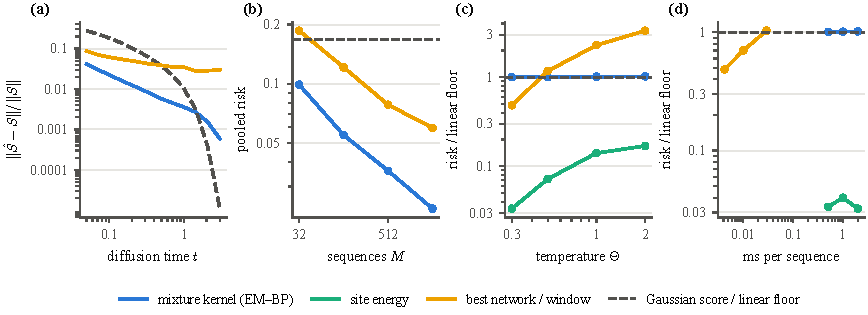
\includegraphics[width=\textwidth]{ff-summary.pdf}
  \caption{\textbf{Summary.} Relative score error against the exact score, pooled over a
  twelve-level noise schedule. (a)~Per-level error on the linear chain with Laplace noise
  ($\nseq=2048$ training sequences): the learned kernel (blue) beats the best network (yellow)
  at every level and the Gaussian score (dashed) except at the highest noise levels.
  (b)~Pooled error against the number of training sequences on the same chain.
  (c)~The $\phi^4$ field ($\nseq=2048$): risk divided by the linear (Gaussian) floor against
  temperature $\Temp$; the five-parameter site energy (green) is far below it, the linear-drift
  mixture kernel of (a, b) sits on it, and the window network rises above it when the field is hot.
  (d)~The same ratio against inference time on three lattice spacings at $\Temp=0.3$ (eight
  threads, the largest network variants).}
  \label{fig:summary}
\end{figure*}

\paragraph{Two laboratories with exact scores.}
The framework is stated for a general kernel (\cref{sec:setup}); we test it on two concrete
cases chosen because their scores can be computed exactly and compared with everything else.
The first is a linear chain with non-Gaussian driving noise, whose covariance is fixed by two
numbers and whose shape by the noise law, so Gaussian, Laplace, Student-$t$, uniform and
bimodal noise share one covariance exactly and differ only in higher-order structure; it
separates, by construction, what diffusion noise does to correlation from what it does to
shape (\cref{sec:experiments}). The second is the one-dimensional $\phi^4$ field, the
stochastic Allen--Cahn model, whose lattice snapshots are exactly Markov, whose kernel is
nonlinear (a double well with domains and kinks), and which has a physical vocabulary
(temperature, correlation length, kink density) and exact transfer-matrix references
(\cref{sec:field}).

\paragraph{Contributions.}
\begin{enumerate}[label=(\roman*),leftmargin=1.6em,itemsep=0.1em,topsep=0.2em]
\item \emph{Exact denoising for any Markov kernel.} Score estimation for Markov data reduces
to posterior means, which BP computes exactly up to a quadrature we measure
(\cref{sec:inference}); the Gaussian kernel is a clean sanity check, since BP with Gaussian
messages is the linear score and the Kalman smoother (\cref{prop:lmmse,prop:kalman};
\cref{sec:sanity}).
\item \emph{The kernel is learnable from noise, and learning it works.} EM through the same
sweep recovers the kernel from one noised view per sequence (\cref{sec:learning}). With a kernel of
a few parameters it beats the neural denoisers it is compared with (six on the linear chain, two on the field) at every sample
size, by a paired factor $\matchedRatioBestD$ at EM--BP's own information interface on the linear chain and by
$\fldNetRatioMin$--$\fldNetRatioMax$ on the field (the best network over the site energy at $\nseq=2048$).
\item \emph{The kernel family is the real modelling choice.} The linear-drift mixture is
exactly right for the linear chain and sits on the linear floor on the field; the
five-parameter site energy, the physicist's pair energy, is best on every field cell; an
unrestricted or neural kernel earns its parameters only where the simple family is
misspecified (\cref{sec:field,sec:limits}).
\item \emph{Cost and limits, measured.} BP is slower per sequence than a network; a coarser grid
recovers most of the gap for the field kernels, and a Fourier representation of the messages
is not worth building (\cref{sec:compute}). A latent shared by a whole sequence leaves a bias
that no sample size removes, which augmenting the state repairs (\cref{sec:limits}).
\end{enumerate}

\paragraph{Supporting theory: what noise erases.}
Why structure matters most where the noise has not yet erased it is a general fact about the
Ornstein--Uhlenbeck channel, and we prove it in the laboratory where it can be checked: the
channel attenuates the Hermite moment of degree $m$ by $e^{-mt}$ exactly, so the Fisher
information a noised sequence carries about a feature first visible at degree $m$ decays as
$e^{-2mt}$ with an explicit constant (correlation as $e^{-4t}$, non-Gaussian shape as $e^{-8t}$),
and the gap between the true score and that of the covariance-matched Gaussian is
$\tfrac16\lVert\kappa_4\rVert_F^2e^{-8t}$ (\cref{sec:theory}). We treat this as supporting
rather than central: it explains where the structured estimator gains, not why it is exact.

\section{Setting: a Markov chain with a general kernel}
\label{sec:setup}

\paragraph{Data.}
A clean sequence $\va\in\Reals^{\nsites}$ is a first-order Markov chain with initial law $\mu$ and
transition kernel $\kernel$,
\begin{equation}
  \Pz(\va)=\mu(a_1)\prod_{i=2}^{\nsites}\kernel(a_i\mid a_{i-1}),
  \label{eq:prior}
\end{equation}
where $\kernel(\cdot\mid a)$ is a continuous density for every $a$. Nothing else is assumed in
\cref{sec:inference,sec:sanity,sec:learning}; stationarity, symmetry and reversibility are
properties of the examples below, not of the method. The kernel is the whole model: it is the
one function from which the law of every site, every pair of sites and the whole sequence
follows. We write $\Reals$ for the state space and $\nsites$ for the chain length; the
ambient dimension is $\nsites$, and $\nseq$ denotes the number of observed sequences.

\paragraph{The channel.}
The forward process is the coordinatewise Ornstein--Uhlenbeck channel
\begin{equation}
  \vx_t = e^{-t}\va + \sqrt{\Dt}\,\vz,\qquad \Dt=1-e^{-2t},\quad \vz\sim\normal{0}{\Id},
  \label{eq:channel}
\end{equation}
so that $\vx_t$ is a noised copy of the same sequence at level $t$. $\Pt$ is its law, and
the score is $\score(\vx,t)=\nabla_{\vx}\log\Pt(\vx)$.

\paragraph{First instance: a linear chain with non-Gaussian noise.}
The simplest kernel with a nontrivial score is a linear one with non-Gaussian driving noise,
\begin{equation}
  \kernel(a'\mid a)=\innov(a'-\corr a),\qquad a_1\sim\normal{0}{1},\quad |\corr|<1,
  \label{eq:linear}
\end{equation}
with a driving-noise density $\innov$ of mean zero and variance $\ivar=1-\corr^2$. The
variance choice makes $\Var(a_i)=1$ and $\Cov(a_i,a_j)=\corr^{|i-j|}$ exactly for \emph{every}
noise law, so the families we use---Gaussian, Laplace, Student-$t$, uniform, a symmetric
two-component mixture, and the generalised Gaussian
$\innov(\varepsilon)\propto\exp(-|\varepsilon/s_\beta|^\beta)$ whose exponent $\beta$ moves the
excess kurtosis from $+3$ (Laplace) through $0$ (Gaussian) to $-1$ at $\beta=6$, at fixed
variance---share one covariance $\Sig_0$ and, every noise law being symmetric, differ only through
cumulants of order four and higher. The laboratory therefore separates, by construction, what
diffusion noise does to correlation from what it does to shape. Throughout \cref{sec:experiments}
the frozen configuration is $\corr=0.85$, $\nsites=32$, Laplace noise.

\paragraph{Second instance: a physical field.}
The one-dimensional $\phi^4$ field is the stochastic Allen--Cahn equation
$\partial_\tau\phi=\partial_s^2\phi-V'(\phi)+\sqrt{2\Temp}\,\eta$ with the double well
$V(\phi)=(\phi^2-1)^2/4$ at temperature $\Temp$; its stationary law is the Gibbs measure
$\propto e^{-H[\phi]/\Temp}$ with $H[\phi]=\int[\tfrac12(\partial_s\phi)^2+V(\phi)]\,\mathrm{d}s$.
On a lattice of spacing $\latt$ the energy couples only nearest neighbours,
$H_{\latt}=\sum_i[(\phi_{i+1}-\phi_i)^2/2\latt+\latt V(\phi_i)]$, so a spatial snapshot is
\emph{exactly} a first-order Markov chain in the site index, with a kernel of the form
\emph{Gaussian step times a function of the arrival point},
\begin{equation}
  \begin{aligned}
  \kernel(\phi'\mid\phi)&=\frac{\normal{\phi';\phi}{\Temp\latt}\,g(\phi')}{Z(\phi)},\\
  Z(\phi)&=\int\normal{\phi';\phi}{\Temp\latt}\,g(\phi')\dd\phi',
  \end{aligned}
  \label{eq:tilted}
\end{equation}
with $g=\psi_0e^{-\latt V/2\Temp}$ built from the leading eigenfunction $\psi_0$ of the symmetric
transfer operator $\transfer(\phi,\phi')=e^{-\latt V(\phi)/2\Temp}e^{-(\phi'-\phi)^2/2\Temp\latt}e^{-\latt V(\phi')/2\Temp}$
(\cref{app:field}). Two knobs set the chain: the temperature $\Temp$ and the spacing $\latt$;
the correlation length in sites is $\corrlen=1/\log(\lambda_0/\lambda_1)$. There is no phase
transition in one dimension: $\corrlen$ is finite at every $\Temp>0$ and grows roughly like
$e^{E_{\mathrm{kink}}/\Temp}$ as $\Temp$ falls, a sharp crossover. Unlike
\cref{eq:linear}, the field's expected next value is a nonlinear function of the current one,
and its driving noise is state-dependent; the two families meet only at the Gaussian chain
(\cref{app:field}). Snapshots are standardised to unit variance, $a=\phi/\sqrt{\operatorname{Var}\phi}$.

\paragraph{What is scored.}
For an estimator $\hat\score$ the \emph{risk} is the relative root-mean-square score error
against the exact score, summed over test chains, sites and the schedule of noise levels
(\cref{app:protocol}). Three reference points bracket every estimator: the isotropic score
$-\vx$, which ignores the chain; the linear (LMMSE) score of the true covariance, which by
\cref{prop:lmmse} is what any second-order estimator can reach; and the exact score, at zero
(\cref{app:oracles}).

\section{What survives diffusion noise: attenuation by statistical order}
\label{sec:theory}

Write $\gamma$ for the standard Gaussian on $\Reals^{\nsites}$, $\Hen{k}$ for the
probabilists' Hermite polynomials and $H_\nu(\vx)=\prod_i\Hen{\nu_i}(x_i)$ for their
products, of degree $|\nu|$. The channel \cref{eq:channel} acts on Hermite moments
diagonally.

\begin{theorem}[Hermite attenuation]
\label{thm:hermite}
For every multi-index $\nu$ with $\E_{\Pz}|\va|^{|\nu|}<\infty$,
$\;\E_{\Pt}[H_\nu(\vx_t)]=e^{-|\nu|t}\,\E_{\Pz}[H_\nu(\va)]$.
\end{theorem}
\begin{proof}
Mehler's identity $\E_{z}[\Hen{n}(\alpha a+\sqrt{1-\alpha^2}\,z)]=\alpha^n\Hen{n}(a)$ for
$z\sim\normal{0}{1}$ follows from the generating function
$e^{sx-s^2/2}=\sum_n\Hen{n}(x)s^n/n!$; coordinates are independent given $\va$, and
$\alpha=e^{-t}$.
\end{proof}
Nothing here requires $\Pz/\gamma\in L^2(\gamma)$---which fails for the Laplace chain and,
because $\lmax(\Sig_0)>2$, for the Gaussian chain at $\corr=0.85$---only finite moments.
Two consequences are exact at every $t$: cumulants of order $m\ge3$ scale as $e^{-mt}$
(Gaussian noise has none), and the degree-4 Hermite moments of two variance-matched laws
differ exactly by their fourth-cumulant tensors $\kfour$, attenuated by $e^{-4t}$.
Correlation lives at degree two and decays as $e^{-2t}$; non-Gaussian shape first appears
at degree four and decays as $e^{-4t}$. \emph{Diffusion noise is a low-pass filter on
statistical order.}

The consequence for scores and for learning is an expansion in the signal-to-noise
ratio $e^{-2t}$. Let $s=e^{-t}\vx/\Dt$, $b=e^{-2t}/\Dt$ and
$\Lambda(s,b)=\log\E_{\Pz}\exp(s\cdot\va-b|\va|^2/2)$, so that
$\log\Pt(\vx)=\log\gamma_{\Dt}(\vx)+\Lambda(s,b)$ and
$\score=-\vx/\Dt+(e^{-t}/\Dt)\nabla_s\Lambda$ exactly. Grading $\Lambda$ by order in
$e^{-t}$, its second-order part is the same for $\Pz$ and its covariance twin, and its
fourth-order part differs by a term linear in $\kfour$.

\begin{theorem}[Order-by-order information decay]
\label{thm:decay}
Let $\Pz$ have finite eighth moments and covariance $\Sig_0$, let $\Sgauss$ be the score
of its covariance twin, and let $\lmax=\lmax(\Sig_0)$. As $t\to\infty$,
\begin{align}
  \E_{\Pt}\lVert\score-\Sgauss\rVert^2
   &= \tfrac{1}{6}\Frob{\kfour}^2\,e^{-8t}\bigl(1+\epsilon_t\bigr),
  \label{eq:scoregap}\\
  I_t(\theta)&= \tfrac12\Frob{\partial_\theta\Sig_0}^2\,e^{-4t}\bigl(1+\epsilon_t\bigr)
  \ \ \text{if }\partial_\theta\Sig_0\neq0,
  \label{eq:info2}\\
  I_t(\theta)&= \tfrac1{24}\Frob{\partial_\theta\kfour}^2\,e^{-8t}\bigl(1+\epsilon_t\bigr)
  \ \ \text{if }\partial_\theta\Sig_0=0,\ \partial_\theta\kfour\neq0,
  \label{eq:info4}
\end{align}
with $\epsilon_t=O(e^{-2t}\lmax)$,
where $I_t(\theta)=\E_{\Pt}[(\partial_\theta\log\Pt)^2]$ is the Fisher information one
noised sequence carries about a parameter $\theta$ of $\Pz$, and $\Frob{\cdot}$ is the
Frobenius norm of the matrix or symmetric 4-tensor. For a Gaussian chain
\cref{eq:info2} is exact at every $t$ with
$I_t=\tfrac12\operatorname{tr}(\Sig_t^{-1}\partial_\theta\Sig_t\Sig_t^{-1}\partial_\theta\Sig_t)$.
\end{theorem}
The information statements \cref{eq:info2,eq:info4} are the diffusion-time form of a
principle established for low-SNR latent-variable models: the log-likelihood expands in
powers of the SNR with the order-$k$ term carrying $k$-th-moment information
\citep{katsevich2023likelihood,perry2019sample,bandeira2023estimation}, and Fisher
information about directions first identifiable at moment order $k$ scales as
$\mathrm{SNR}^k$ \citep{balanov2026gmm}; with $\mathrm{SNR}_t\simeq e^{-2t}$ these are
\cref{eq:info2,eq:info4}. The cumulant attenuation behind \cref{thm:hermite} is also
written down for the forward process by \citet{aarts2025cumulants}. What is new is
the score-level statement \cref{eq:scoregap} with its constant, made interpretable by
\cref{prop:lmmse}; the crossover below; and the exact verification and learning
consequences that follow. The proof (\cref{app:proofs}) expands $\Lambda$ to fourth order, takes the
$\gamma$-second moment of the leading Hermite term by Wick's theorem, and bounds the
remainder by the moment condition; the scalar leading term of \cref{eq:scoregap} is
$(\kfour/6)\Hen{3}(x)e^{-4t}$. The leading orders of a degree-2 and a degree-4 coordinate
do not couple, because $\Hen{2}$ and $\Hen{4}$ are $\gamma$-orthogonal, so the
\emph{efficient} information of a shape coordinate after the nuisance coordinates are
estimated has the same rate as its raw information.

\begin{remark}[General order]
The same grading gives, for a coordinate whose lowest non-vanishing Hermite footprint has
degree $m$, $I_t(\theta)\propto e^{-2mt}$: the leading term of $\partial_\theta\log\Pt$ is
$e^{-mt}$ times a degree-$m$ Hermite polynomial, whose $\gamma$-second moment is a
constant. The constants are explicit for $m=2,4$ above.
\end{remark}

\begin{corollary}[Sample complexity by order]
\label{cor:samples}
Estimating a covariance coordinate to fixed precision from sequences observed at level
$t$ needs $\nseq\propto e^{4t}$ of them; a shape coordinate needs $\nseq\propto e^{8t}$.
The ratio of the two informations is $\propto e^{-4t}$.
\end{corollary}

\paragraph{Where the asymptote begins.}
The expansion parameter is $e^{-2t}\lmax(\Sig_0)$, not $e^{-2t}$, with
$\lmax\le(1+\corr)/(1-\corr)$ for the chain. Below
$\tstar=\tfrac12\log\lmax(\Sig_0)$ the long-wavelength covariance modes are still of
order one and the rates are shallower; above it the exponents of \cref{thm:decay} hold.
At $\corr=0.85$, $\tstar=\gaussTstareightfive$: a strongly correlated chain keeps its
correlation information longer, and any measurement stopped near $\tstar$ sees slopes
short of $-4$ and $-8$.

\begin{figure*}[t]
  \centering
  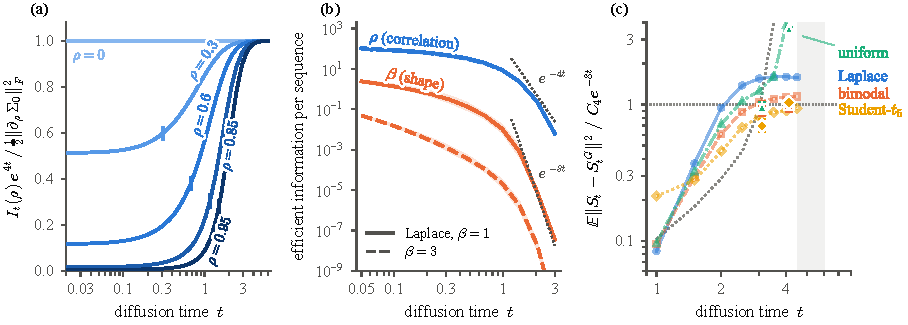
\includegraphics[width=\textwidth]{fig_theory.pdf}
  \caption{\textbf{What survives diffusion noise.}
  (a)~Exact Fisher information of the Gaussian chain about $\corr$, scaled by its
  predicted asymptote $\tfrac12\Frob{\partial_\corr\Sig_0}^2e^{-4t}$, for five $\corr$;
  every curve reaches~1, and the tick on each marks $\tstar(\corr)$.
  (b)~Efficient information per noised sequence about the correlation coordinate $\corr$
  (degree~2) and the shape coordinate $\beta$ (degree~4) of the generalised-Gaussian
  chain, from tree-exact inference and Fisher's identity, $\shapeChains$ sequences
  $\times\,\shapeReps$ replicates (bands: replicate range); guides $e^{-4t}$ and $e^{-8t}$.
  Above $\tstar$ the fitted slopes are $\shapeSlopeRhoone$ ($\corr$) and
  $\shapeSlopeBetathree$ ($\beta$, at $\beta=3$).
  (c)~The price of second-order closure: $\E\lVert\score-\Sgauss\rVert^2$ measured by
  tree-exact BP, divided by the predicted $\tfrac16\Frob{\kfour}^2e^{-8t}$, for four
  innovation families. Laplace and the bimodal mixture reach the constant to within
  $\closureRatiolaplacetthreepzero$--$\closureRatiobimodaltfourpzero$; Student-$t_5$, whose sixth
  moment is infinite, departs as the moment condition predicts; the uniform family reaches
  the floor of double precision near $t=3.5$.}
  \label{fig:theory}
\end{figure*}

\paragraph{Verification with the exact score.}
\Cref{fig:theory} tests \cref{thm:decay} where nothing has to be approximated. For the
Gaussian chain the closed form gives slope $\gaussSlopeRhoeightfive$ above $\tstar$ at
$\corr=0.85$ and the scaled information $\gaussScaledRhoeightfivetone$, $\gaussScaledRhoeightfivettwo$,
$\gaussScaledRhoeightfivetthree$ at $t=1,2,3$. For the non-Gaussian chain the shape information,
estimated from per-sequence scores obtained by Fisher's identity through the tree-exact
recursion, falls with slope $\shapeSlopeBetatwo$ ($\beta=2$) and $\shapeSlopeBetathree$
($\beta=3$) above $\tstar$, against the predicted $-8$, while the correlation
information falls with slope $\shapeSlopeRhotwo$ against $-4$; the kinked Laplace density
($\beta=1$) reaches the quadrature floor of the outer-product estimate near $t=2.5$.
The closure gap on the Laplace chain decays with slope $\closureSlopeSqlaplace$ and
reproduces the constant $\tfrac16\Frob{\kfour}^2$ ($\closureCfourlaplace$ for
$\nsites=32$) to $\closureRatiolaplacetthreepzero$ at $t=3$. The theorem also explains a
measurement the previous literature on this model reported as a discrepancy: information
slopes of about $-3$ and $-6$ obtained over $t\le1.6$ are the pre-asymptotic values below
$\tstar=\gaussTstareightfive$, not a failure of the $e^{-4t}$, $e^{-8t}$ law.

\paragraph{What this says about score learning.}
An estimator that carries only second-order structure cannot go below the LMMSE floor
$\lVert\score-\Sgauss\rVert$, which on the Laplace chain at $\corr=0.85$ is
$\lmmseFloorLaplace$ of the score energy pooled over the twelve-level schedule and
$\lmmseLowestLaplace$ at the lowest level (\cref{app:oracles}). A learner that recovers the
fourth-order structure has, by \cref{cor:samples}, $e^{4t}$ fewer effective samples per
sequence at level $t$ than one that recovers only covariance: the twelve-level schedule
is, for shape, effectively a four-level one. Both facts organise the experiments of
\cref{sec:experiments}.

\section{Learning the local law through noise}
\label{sec:learning}

Now drop the assumption that $\kernel$ is known. We observe $\nseq$ noised sequences
$\vx^{\mu}$, each at one level $t_\mu$, never the clean chain, and maximise the marginal
log-likelihood $\Lik(\params)=\sum_\mu\log\Pt[t_\mu,\params](\vx^\mu)$ of a parameterised kernel
$\kernelth$. Because \cref{sec:inference} computes this likelihood and its gradient exactly,
learning the kernel and inferring the posterior are the same recursion.

\paragraph{The exact gradient from one sweep.}
Because only the transition factors depend on $\params$, Fisher's identity
\citep{cappe2005} gives, on the grid,
\begin{equation}
\begin{aligned}
  \nabla_\params\Lik(\params)&=\bigl\langle\Xis(\params),\,\nabla_\params\log\kernelth\bigr\rangle,\\
  \Xis_{kl}&=\sum_{\mu}\sum_{i\ge2}P(a_i=\gridpt{k},a_{i-1}=\gridpt{l}\mid\vx^\mu),
\end{aligned}
\label{eq:fisher}
\end{equation}
where the expected transition mass $\Xis$ is read off the pairwise marginals that the same
forward--backward pass returns. No differentiation through the recursion is needed, and the identity
is verified against finite differences and against brute-force enumeration of the evidence on short
chains (\codefile{tests/test\_em\_bp.py}, \codefile{tests/test\_fisher\_bruteforce.py}). $\Xis$ is also all
the M-step of EM needs, so EM alternates the two halves of \cref{fig:method}: run BP with the current
kernel to get $\Xis$ (E-step), refit the kernel to $\Xis$ (M-step). The estimator sees one frozen
noised view per sequence and never a clean trajectory; each reported fit selects its iteration
count on a validation bundle disjoint from the test bundle, by the held-out risk against the exact score
or, with no true score anywhere, by the held-out one-view log-evidence (\cref{app:protocol}).

\paragraph{The kernel families.}
The M-step depends on how the kernel is parameterised, and the choice is the main modelling decision.
\begin{itemize}[leftmargin=1.2em,itemsep=0.1em,topsep=0.2em]
\item \emph{Mixture kernel} (25 numbers). For the linear chain,
$\kernelth(a'\mid a)=\sum_{c=1}^{\ncomp}\pi_c\,\normal{a'-\corr a-\nu_c}{s_c^2}$: a linear drift with
driving noise an $\ncomp$-component Gaussian mixture. $\ncomp=1$ is the linear-Gaussian kernel and recovers
the Gaussian score (\cref{prop:lmmse}); $\ncomp=8$ is the paper's estimator. For $\corr$ it is the
belief-weighted Yule--Walker pair $\corr=S_{01}/S_{00}$, $\ivar=(S_{11}-\corr S_{01})/W$ with
$S_{00}=\sum_{kl}\Xis_{kl}\gridpt{l}^2$, $S_{01}=\sum_{kl}\Xis_{kl}\gridpt{k}\gridpt{l}$,
$S_{11}=\sum_{kl}\Xis_{kl}\gridpt{k}^2$ and $W=\sum_{kl}\Xis_{kl}$; the complete-data problem for the
mixture carries a second latent label and we take conditional-maximisation sweeps, a generalised EM
whose ascent is monotone \citep{dempster1977maximum,meng1993maximum}.
\item \emph{Tilted-walk kernels} (7, 25 numbers). For a nonlinear drift,
$\kernelth(a'\mid a)=\normal{a';a}{\bondvar}\,e^{B(a')\cdot\params}/Z_\params(a)$, a Gaussian step with a
learned tilt of the arrival point, $B$ a Legendre or cubic-spline basis. It contains the field's kernel
\cref{eq:tilted} exactly, and the M-step objective is concave in $\params$ at fixed $\bondvar$.
\item \emph{The site energy} (5 numbers). Every tilted walk is reversible with the symmetric pair energy
$W(a,a')=(a'-a)^2/2\bondvar+f(a)+f(a')$, so the directed kernel and the pair energy are one model class
(\cref{app:field}). Parameterising $f$ as a quartic polynomial and $\bondvar$ gives five numbers,
exactly specified for the $\phi^4$ field, and a fitted kernel reads as physics: the temperature
$\hat\Temp=\hat\bondvar s^2/\latt$, the barrier height and the well position.
\item \emph{Unrestricted and neural kernels} (100 and 1\,516 numbers). A log-linear kernel with a free
two-dimensional spline for $\log\kernel$, which assumes no Gaussian bond, and a mixture density network
(MDN) that maps $a$ to a Gaussian mixture for $a'$. Both are fitted by the same EM; they are the tools for
asking whether a simple family is wide enough (\cref{sec:limits}).
\end{itemize}

\paragraph{Resolution and capacity.}
A flexible kernel can learn narrow features, and the grid must resolve them: with large $\ncomp$ and many
sequences the mixture's narrowest component can be finer than a coarse grid's spacing, which we measure
through a ``resolved'' flag (\cref{sec:compute}). The structure is not free either: $\ncomp=1$ cannot see
fourth-order structure and a large kernel overfits, which is why the tilted and site-energy families have
few parameters.

\section{A controlled laboratory: the linear chain with non-Gaussian noise}
\label{sec:experiments}

The linear chain of \cref{eq:linear} is the cleanest place to ask what structure is worth, because its
covariance is fixed by two numbers and everything beyond it by the noise law, and because its exact score is
available. We ask three things: what diffusion noise erases, and when (\cref{sec:theory}); whether the
kernel can be learned through that noise (\cref{sec:learning-results}); and what explicit structure buys
against networks (\cref{sec:buys}). Where it stops is \cref{sec:limits}. All comparisons use the frozen
configuration of \cref{app:protocol}: Laplace noise, $\corr=0.85$, $\nsites=32$, twelve log-spaced levels on
$[0.05,3]$, and the schedule-pooled relative score error against the tree-exact reference. Paired seeds are
the inferential unit, sixteen at the frozen configuration and eight in the sweeps across regimes; every
selection is made on development seeds or on a validation bundle that never enters a reported number.
Three information interfaces are distinguished throughout: (A) the standard denoising recipe, clean sequences
with a fresh corruption at every step; (B) clean sequences with one fixed corruption each; (C) one noised
view per sequence and nothing else, which is what EM--BP sees. Three reference points bracket every estimator
(\cref{app:oracles}): the isotropic score $-\vx$ at $\isoFloorLaplace$, the LMMSE oracle with the true
covariance at $\lmmseFloorLaplace$, the floor of every second-order estimator by \cref{prop:lmmse}, and the
exact score at zero.

\section{What survives diffusion noise: attenuation by statistical order}
\label{sec:theory}

Write $\gamma$ for the standard Gaussian on $\Reals^{\nsites}$, $\Hen{k}$ for the
probabilists' Hermite polynomials and $H_\nu(\vx)=\prod_i\Hen{\nu_i}(x_i)$ for their
products, of degree $|\nu|$. The channel \cref{eq:channel} acts on Hermite moments
diagonally.

\begin{theorem}[Hermite attenuation]
\label{thm:hermite}
For every multi-index $\nu$ with $\E_{\Pz}|\va|^{|\nu|}<\infty$,
$\;\E_{\Pt}[H_\nu(\vx_t)]=e^{-|\nu|t}\,\E_{\Pz}[H_\nu(\va)]$.
\end{theorem}
\begin{proof}
Mehler's identity $\E_{z}[\Hen{n}(\alpha a+\sqrt{1-\alpha^2}\,z)]=\alpha^n\Hen{n}(a)$ for
$z\sim\normal{0}{1}$ follows from the generating function
$e^{sx-s^2/2}=\sum_n\Hen{n}(x)s^n/n!$; coordinates are independent given $\va$, and
$\alpha=e^{-t}$.
\end{proof}
Nothing here requires $\Pz/\gamma\in L^2(\gamma)$---which fails for the Laplace chain and,
because $\lmax(\Sig_0)>2$, for the Gaussian chain at $\corr=0.85$---only finite moments.
Two consequences are exact at every $t$: cumulants of order $m\ge3$ scale as $e^{-mt}$
(Gaussian noise has none), and the degree-4 Hermite moments of two variance-matched laws
differ exactly by their fourth-cumulant tensors $\kfour$, attenuated by $e^{-4t}$.
Correlation lives at degree two and decays as $e^{-2t}$; non-Gaussian shape first appears
at degree four and decays as $e^{-4t}$. \emph{Diffusion noise is a low-pass filter on
statistical order.}

The consequence for scores and for learning is an expansion in the signal-to-noise
ratio $e^{-2t}$. Let $s=e^{-t}\vx/\Dt$, $b=e^{-2t}/\Dt$ and
$\Lambda(s,b)=\log\E_{\Pz}\exp(s\cdot\va-b|\va|^2/2)$, so that
$\log\Pt(\vx)=\log\gamma_{\Dt}(\vx)+\Lambda(s,b)$ and
$\score=-\vx/\Dt+(e^{-t}/\Dt)\nabla_s\Lambda$ exactly. Grading $\Lambda$ by order in
$e^{-t}$, its second-order part is the same for $\Pz$ and its covariance twin, and its
fourth-order part differs by a term linear in $\kfour$.

\begin{theorem}[Order-by-order information decay]
\label{thm:decay}
Let $\Pz$ have finite eighth moments and covariance $\Sig_0$, let $\Sgauss$ be the score
of its covariance twin, and let $\lmax=\lmax(\Sig_0)$. As $t\to\infty$,
\begin{align}
  \E_{\Pt}\lVert\score-\Sgauss\rVert^2
   &= \tfrac{1}{6}\Frob{\kfour}^2\,e^{-8t}\bigl(1+\epsilon_t\bigr),
  \label{eq:scoregap}\\
  I_t(\theta)&= \tfrac12\Frob{\partial_\theta\Sig_0}^2\,e^{-4t}\bigl(1+\epsilon_t\bigr)
  \ \ \text{if }\partial_\theta\Sig_0\neq0,
  \label{eq:info2}\\
  I_t(\theta)&= \tfrac1{24}\Frob{\partial_\theta\kfour}^2\,e^{-8t}\bigl(1+\epsilon_t\bigr)
  \ \ \text{if }\partial_\theta\Sig_0=0,\ \partial_\theta\kfour\neq0,
  \label{eq:info4}
\end{align}
with $\epsilon_t=O(e^{-2t}\lmax)$,
where $I_t(\theta)=\E_{\Pt}[(\partial_\theta\log\Pt)^2]$ is the Fisher information one
noised sequence carries about a parameter $\theta$ of $\Pz$, and $\Frob{\cdot}$ is the
Frobenius norm of the matrix or symmetric 4-tensor. For a Gaussian chain
\cref{eq:info2} is exact at every $t$ with
$I_t=\tfrac12\operatorname{tr}(\Sig_t^{-1}\partial_\theta\Sig_t\Sig_t^{-1}\partial_\theta\Sig_t)$.
\end{theorem}
The information statements \cref{eq:info2,eq:info4} are the diffusion-time form of a
principle established for low-SNR latent-variable models: the log-likelihood expands in
powers of the SNR with the order-$k$ term carrying $k$-th-moment information
\citep{katsevich2023likelihood,perry2019sample,bandeira2023estimation}, and Fisher
information about directions first identifiable at moment order $k$ scales as
$\mathrm{SNR}^k$ \citep{balanov2026gmm}; with $\mathrm{SNR}_t\simeq e^{-2t}$ these are
\cref{eq:info2,eq:info4}. The cumulant attenuation behind \cref{thm:hermite} is also
written down for the forward process by \citet{aarts2025cumulants}. What is new is
the score-level statement \cref{eq:scoregap} with its constant, made interpretable by
\cref{prop:lmmse}; the crossover below; and the exact verification and learning
consequences that follow. The proof (\cref{app:proofs}) expands $\Lambda$ to fourth order, takes the
$\gamma$-second moment of the leading Hermite term by Wick's theorem, and bounds the
remainder by the moment condition; the scalar leading term of \cref{eq:scoregap} is
$(\kfour/6)\Hen{3}(x)e^{-4t}$. The leading orders of a degree-2 and a degree-4 coordinate
do not couple, because $\Hen{2}$ and $\Hen{4}$ are $\gamma$-orthogonal, so the
\emph{efficient} information of a shape coordinate after the nuisance coordinates are
estimated has the same rate as its raw information.

\begin{remark}[General order]
The same grading gives, for a coordinate whose lowest non-vanishing Hermite footprint has
degree $m$, $I_t(\theta)\propto e^{-2mt}$: the leading term of $\partial_\theta\log\Pt$ is
$e^{-mt}$ times a degree-$m$ Hermite polynomial, whose $\gamma$-second moment is a
constant. The constants are explicit for $m=2,4$ above.
\end{remark}

\begin{corollary}[Sample complexity by order]
\label{cor:samples}
Estimating a covariance coordinate to fixed precision from sequences observed at level
$t$ needs $\nseq\propto e^{4t}$ of them; a shape coordinate needs $\nseq\propto e^{8t}$.
The ratio of the two informations is $\propto e^{-4t}$.
\end{corollary}

\paragraph{Where the asymptote begins.}
The expansion parameter is $e^{-2t}\lmax(\Sig_0)$, not $e^{-2t}$, with
$\lmax\le(1+\corr)/(1-\corr)$ for the chain. Below
$\tstar=\tfrac12\log\lmax(\Sig_0)$ the long-wavelength covariance modes are still of
order one and the rates are shallower; above it the exponents of \cref{thm:decay} hold.
At $\corr=0.85$, $\tstar=\gaussTstareightfive$: a strongly correlated chain keeps its
correlation information longer, and any measurement stopped near $\tstar$ sees slopes
short of $-4$ and $-8$.

\begin{figure*}[t]
  \centering
  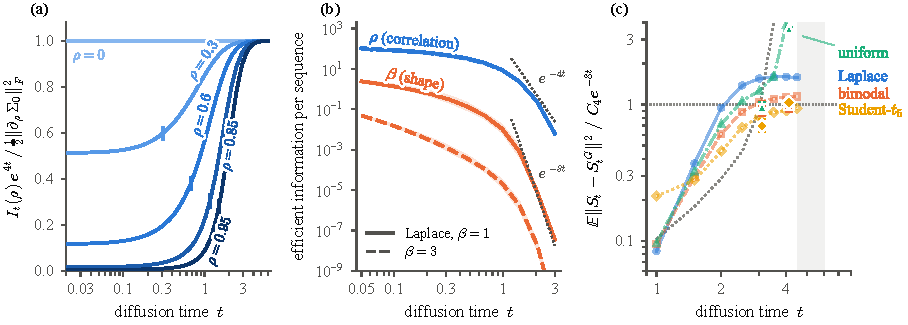
\includegraphics[width=\textwidth]{fig_theory.pdf}
  \caption{\textbf{What survives diffusion noise.}
  (a)~Exact Fisher information of the Gaussian chain about $\corr$, scaled by its
  predicted asymptote $\tfrac12\Frob{\partial_\corr\Sig_0}^2e^{-4t}$, for five $\corr$;
  every curve reaches~1, and the tick on each marks $\tstar(\corr)$.
  (b)~Efficient information per noised sequence about the correlation coordinate $\corr$
  (degree~2) and the shape coordinate $\beta$ (degree~4) of the generalised-Gaussian
  chain, from tree-exact inference and Fisher's identity, $\shapeChains$ sequences
  $\times\,\shapeReps$ replicates (bands: replicate range); guides $e^{-4t}$ and $e^{-8t}$.
  Above $\tstar$ the fitted slopes are $\shapeSlopeRhoone$ ($\corr$) and
  $\shapeSlopeBetathree$ ($\beta$, at $\beta=3$).
  (c)~The price of second-order closure: $\E\lVert\score-\Sgauss\rVert^2$ measured by
  tree-exact BP, divided by the predicted $\tfrac16\Frob{\kfour}^2e^{-8t}$, for four
  innovation families. Laplace and the bimodal mixture reach the constant to within
  $\closureRatiolaplacetthreepzero$--$\closureRatiobimodaltfourpzero$; Student-$t_5$, whose sixth
  moment is infinite, departs as the moment condition predicts; the uniform family reaches
  the floor of double precision near $t=3.5$.}
  \label{fig:theory}
\end{figure*}

\paragraph{Verification with the exact score.}
\Cref{fig:theory} tests \cref{thm:decay} where nothing has to be approximated. For the
Gaussian chain the closed form gives slope $\gaussSlopeRhoeightfive$ above $\tstar$ at
$\corr=0.85$ and the scaled information $\gaussScaledRhoeightfivetone$, $\gaussScaledRhoeightfivettwo$,
$\gaussScaledRhoeightfivetthree$ at $t=1,2,3$. For the non-Gaussian chain the shape information,
estimated from per-sequence scores obtained by Fisher's identity through the tree-exact
recursion, falls with slope $\shapeSlopeBetatwo$ ($\beta=2$) and $\shapeSlopeBetathree$
($\beta=3$) above $\tstar$, against the predicted $-8$, while the correlation
information falls with slope $\shapeSlopeRhotwo$ against $-4$; the kinked Laplace density
($\beta=1$) reaches the quadrature floor of the outer-product estimate near $t=2.5$.
The closure gap on the Laplace chain decays with slope $\closureSlopeSqlaplace$ and
reproduces the constant $\tfrac16\Frob{\kfour}^2$ ($\closureCfourlaplace$ for
$\nsites=32$) to $\closureRatiolaplacetthreepzero$ at $t=3$. The theorem also explains a
measurement the previous literature on this model reported as a discrepancy: information
slopes of about $-3$ and $-6$ obtained over $t\le1.6$ are the pre-asymptotic values below
$\tstar=\gaussTstareightfive$, not a failure of the $e^{-4t}$, $e^{-8t}$ law.

\paragraph{What this says about score learning.}
An estimator that carries only second-order structure cannot go below the LMMSE floor
$\lVert\score-\Sgauss\rVert$, which on the Laplace chain at $\corr=0.85$ is
$\lmmseFloorLaplace$ of the score energy pooled over the twelve-level schedule and
$\lmmseLowestLaplace$ at the lowest level (\cref{app:oracles}). A learner that recovers the
fourth-order structure has, by \cref{cor:samples}, $e^{4t}$ fewer effective samples per
sequence at level $t$ than one that recovers only covariance: the twelve-level schedule
is, for shape, effectively a four-level one. Both facts organise the experiments of
\cref{sec:experiments}.


\subsection{Learning the shape and the correlation through noise}
\label{sec:learning-results}

\paragraph{The information curve predicts what is learned at each level.}
\Cref{cor:samples} makes a prediction about learning that the exact score does not need: fitting from
$\nseq$ sequences all observed at level $t$, the shape of the driving-noise law stops being identifiable at
the level where its Cram\'er--Rao reference crosses the coordinate's range, while the correlation survives to
the crossover. This is also the arithmetic behind the one-view protocol: of twelve levels spread over
$t\in[0.05,3]$, only the lowest four carry appreciable information about shape.

\begin{figure}[t]
  \centering
  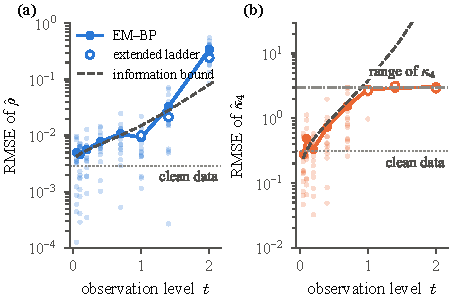
\includegraphics[width=\columnwidth]{fig_learning.pdf}
  \caption{\textbf{Learning through noise.} Recovery of the correlation coordinate and
  of the driving-noise shape from $\nseq=512$ sequences observed at a single level $t$,
  sixteen replicates (points: individual fits; line: RMSE), against the Cram\'er--Rao
  reference (dashed), the clean-data floor (dotted) and, for the shape, the coordinate's
  range. The fits are unimodal and at the reference at the lowest levels, split into a
  shrunk cluster and Gaussian-collapsed fits from $t=\learnLevelTzeropseven$, and collapse
  where the reference crosses the range. Hollow markers: the same fits with the \textsc{em}
  ladder extended to $\learnBudgetLadderMax$ iterations (\textsc{e06c}).}
  \label{fig:learning}
\end{figure}
%% Included by 04-learning.tex only when sections/learning-numbers.tex exists (E06 done).
\Cref{fig:learning} measures both with $\nseq=\learnSize$ Laplace-chain sequences and
$\learnSeeds$ replicates per level. Above $\tstar$ the fitted log-slopes of the two
errors against the observation level are $\learnSlopeRho$ for $\widehat\corr$ and
$\learnSlopeKurt$ for $\widehat\kfour$, against the predicted $2$ and $4$; their
difference, $\learnSlopeRatio$, is the $e^{2t}$ separation of \cref{cor:samples}. At
$t=0.1$ the fitted excess kurtosis is recovered to $\learnRmseKurtTzeropone$ RMSE and
the transition law to Hellinger distance $\learnHellTzeropone$; at $t=2$ the RMSE is
$\learnRmseKurtTtwo$ against a true value of $3$, while $\widehat\corr$ is still within
$\learnRmseRhoTtwo$. The clean-data fit (no channel) gives the optimiser's own floor,
$\learnRmseRhoTzero$ and $\learnRmseKurtTzero$.


\subsection{What explicit structure buys}
\label{sec:buys}

\paragraph{Capacity: the margin is fourth-order.}
%% Included by 05-experiments.tex only when sections/capacity-numbers.tex exists (E02a done).
%% GENERATED by tools/make_capacity_numbers.py from outputs/E02a -- do not hand-edit.
\begin{table}[t]\setlength{\tabcolsep}{4.5pt}
\centering
\small
\caption{Schedule-pooled relative score error on all sites, mean over $\capSeeds$ seeds (s.e.\ in the text macros; the isotropic reference is $\capIsoD$ at every size). Every arm is scored on identical test bundles. The last column is the same capacity fitted to the innovation law itself---the $\ncomp$-component mixture closest in Kullback--Leibler divergence, an infinite-data reference for the family rather than a bound; $\dagger$ marks fits whose narrowest component is under two grid cells.}
\label{tab:capacity}
\begin{tabular}{lcccc|c}
\toprule
& \multicolumn{4}{c|}{sequences $\nseq$} & \\
kernel & $32$ & $128$ & $512$ & $2048$ & $\nseq=\infty$ \\
\midrule
LMMSE floor & 0.167 & 0.167 & 0.167 & 0.167 & 0.167 \\
$\ncomp=1$ & 0.174 & 0.168 & 0.168 & 0.167 & 0.167 \\
$\ncomp=2$ & 0.084 & 0.050 & 0.035 & 0.028 & 0.039 \\
$\ncomp=4$ & 0.093 & 0.053 & 0.037 & 0.025 & 0.0057 \\
$\ncomp=8$ & 0.099 & 0.055 & 0.036 & 0.023 & 0.0022$^{\dagger}$ \\
$\ncomp=16$ & 0.100 & 0.056 & 0.036 & 0.022 & 0.0007$^{\dagger}$ \\
\bottomrule
\end{tabular}
\end{table}

\Cref{tab:capacity} places every arm on identical test bundles. A Gaussian-innovation
kernel ($\ncomp=1$) lands on the LMMSE floor at every size
($\capEmoneA$, $\capEmoneB$, $\capEmoneC$, $\capEmoneD$ against the floor
$\capLmmseA$--$\capLmmseD$), as \cref{prop:lmmse} requires; the mixture kernel goes
far below it, reaching $\capEmeightD$ at $\nseq=2048$, $\capFloorRatioD\times$ under the
floor. The paired $\ncomp=8$ versus $\ncomp=1$ difference is
$\capDiffD$ (bootstrap $[\capDiffDlo,\capDiffDhi]$) at $\nseq=2048$ and
$\capDiffA$ ($[\capDiffAlo,\capDiffAhi]$) already at $\nseq=32$, in favour of the
mixture in $\capWinsD$ and $\capWinsA$ of $\capSeeds$ seeds. The best capacity grows with
the data: $\ncomp=\capBestCapA$ at $\nseq=32$ and $\ncomp=\capBestCapD$ at
$\nseq=2048$, the usual variance-to-bias trade, and at $\nseq=2048$ the $\ncomp=8$ arm is
selected at the top of its iteration ladder in $\capAtCapeightD$ of $\capSeeds$ seeds, so
its error there is an upper bound on what a longer ladder would give. The fitted innovation
excess kurtosis is $\capKurteightD$ at $\nseq=2048$ against the true $3$; $\capUnresolved$
cells fail the two-grid-cell resolution gate and are reported, not dropped. The last row of
\cref{tab:capacity} is the family's infinite-data reference: the $\ncomp$-component mixture
closest in Kullback--Leibler divergence to the Laplace innovation, scored on the same
bundles. Its $\ncomp=1$ member is the covariance twin and scores $\capPopone$, the LMMSE
floor to three decimals, as \cref{prop:lmmse} requires; at $\ncomp=8$ it scores
$\capPopeight$, so the fitted kernel at $\nseq=2048$ sits $\capPopRatioeightD\times$ above
what its own family can express, a data limit rather than a capacity limit. (The reference is
not a bound: a Kullback--Leibler-optimal innovation need not minimise the score error, and
the $\ncomp=2$ fit at $\nseq=2048$ scores below it.)

An earlier study of this model concluded the opposite from a sweep that, it turned out, had fitted
every arm to a single training chain (\cref{app:capacity}); with independent chains and the checkpoint
selected identically for every capacity the effect is unambiguous.
Capacity buys exactly what the closure discards: across the generalised-Gaussian family at fixed
covariance the paired gain of $\ncomp=8$ over $\ncomp=1$ is ordered by $\kfour$,
$\famDiffBone$ at the Laplace member and a small loss, $\famDiffBtwo$, at the Gaussian
member, where there is no fourth-order structure to buy (\cref{app:family}, \cref{fig:family}).
The contrast is not a property of the frozen point: in all $\regCells$ cells of a sweep over
$\corr\in[\regRhoLo,\regRhoHi]$ and $\nsites\in[\regLenLo,\regLenHi]$ the mixture beats
the Gaussian kernel with the paired interval excluding zero, the paired difference
$\ncomp=8$ minus $\ncomp=1$ running from $\regGainStrongest$ at the most favourable corner
to $\regGainWeakest$ at the least, and in every cell the $\ncomp=1$
arm lands on the LMMSE floor to $\regIdentMax$, which checks the whole apparatus away from
the frozen configuration (\cref{app:regimes}).

\paragraph{Baselines under one recipe.}
%% Included by 05-experiments.tex only when sections/baseline-numbers.tex exists (E03 done).
%% GENERATED by tools/make_baseline_numbers.py -- do not hand-edit.
\begin{table*}[t]\centering\small\setlength{\tabcolsep}{4.5pt}
\caption{All-site schedule-pooled relative score error, mean over the confirmatory seeds ($\pm$ s.e.\ in the macros), every arm on identical test bundles. Oracles and EM--BP ($\ncomp=8$) from the capacity experiment; networks under the common recipe with the screened configuration.}
\label{tab:baselines}
\begin{tabular}{@{}rccccccccc@{}}
\toprule
$\nseq$ & isotropic & LMMSE & MLP & window & TCN & bi-GRU & transf. & U-Net & EM--BP \\
\midrule
32 & 0.669 & 0.167 & 0.517 & 0.186 & 0.223 & 0.201 & 0.231 & 0.227 & 0.099 \\
128 & 0.669 & 0.167 & 0.391 & 0.141 & 0.139 & 0.121 & 0.151 & 0.150 & 0.055 \\
512 & 0.669 & 0.167 & 0.276 & 0.121 & 0.096 & 0.078 & 0.097 & 0.095 & 0.036 \\
2048 & 0.669 & 0.167 & 0.208 & 0.118 & 0.068 & 0.060 & 0.063 & 0.066 & 0.023 \\
\bottomrule
\end{tabular}
\end{table*}

\Cref{tab:baselines} compares six architectures trained under one recipe (per-example noise
level, batch $64$, Adam with clipping, both output parameterisations, checkpoint selected on
validation), each with the configuration that won its family's screen on the development
seeds (\cref{tab:screen}, \cref{app:protocol}), on the test bundles of the capacity
experiment. Weight sharing is what separates the architectures at small $\nseq$: the fully
connected network reaches only $\baseWorstA$ at $\nseq=32$ against $\baseBestA$ for the
$\baseBestArchA$. Which shared architecture wins depends on the sample size---the
$\baseBestArchA$ at $\nseq=32$, the $\baseBestArchD$ at $\nseq=2048$---so locality is a
useful prior when sequences are scarce and a constraint when they are not.

Given enough clean sequences the networks pass the second-order floor: at $\nseq=2048$,
$\baseBelowFloorND$ of the six sit below $\baseLmmseD$ (\cref{prop:lmmse}), the best at
$\baseBestD$. They are not held at second order by anything intrinsic; they simply need the
data. The structured estimator is nonetheless ahead at every size---$\capEmeightD$ at
$\nseq=2048$, a paired factor $\baseRatioBestD$
($[\baseRatioBestDlo,\baseRatioBestDhi]$, favouring EM--BP in $\baseWinsBestD$ of
$\baseSeeds$ seeds) below the best network, and $\baseRatioBestA$ at $\nseq=32$---and it is
ahead while seeing strictly less of each sequence, which is what the next paragraph measures.

\paragraph{Information-matched training.}
Trained by implicit score matching on the one-view noisy bundle that EM--BP sees, with the
checkpoint selected on the implicit objective of a held-out noisy bundle and the true score
used only to report, the window head reaches $\matchedIsmoneviewWindowD$ and the transformer
$\matchedIsmoneviewTransformerD$ at $\nseq=2048$; with clean targets but a single fixed
corruption per sequence they reach $\matchedDsmonecorruptionWindowD$ and
$\matchedDsmonecorruptionTransformerD$. The distance between these and the standard-recipe
rows is the value of the clean signal and of fresh corruptions; the distance that remains to
EM--BP at the same interface is the value of the structure.

\paragraph{Length extrapolation.}
%% GENERATED by tools/make_baseline_numbers.py -- do not hand-edit.
\begin{table}[t]\centering\small\setlength{\tabcolsep}{4pt}
\caption{Length extrapolation at $\nseq=2048$: pooled relative score error of estimators fitted at $\nsites=32$ and evaluated against the tree-exact score of longer chains, mean over $\baseSeeds$ seeds. Longer chains are slightly easier (proportionally fewer boundary sites), so a length-agnostic arm should improve a little; the transformer instead breaks down beyond its training length.}
\label{tab:length}
\begin{tabular}{@{}lcccc@{}}
\toprule
arm & $\nsites=32$ & $\nsites=64$ & $\nsites=128$ & $\nsites=256$ \\
\midrule
bi-GRU & 0.060 & 0.057 & 0.057 & 0.056 \\
EM--BP & 0.023 & 0.023 & 0.023 & 0.023 \\
TCN & 0.068 & 0.066 & 0.065 & 0.064 \\
transf. & 0.063 & 0.243 & 0.514 & 0.703 \\
U-Net & 0.066 & 0.064 & 0.062 & 0.062 \\
window & 0.118 & 0.099 & 0.088 & 0.082 \\
\bottomrule
\end{tabular}
\end{table}

Fitted at $\nsites=32$ and evaluated at $\nsites=256$, the EM--BP kernel's error moves from
$\lenEmbpDLthreetwo$ to $\lenEmbpDLtwofivesix$: the learned law is local and the inference is
exact at any length. The window head, also local, moves from $\lenWindowDLthreetwo$ to
$\lenWindowDLtwofivesix$; the transformer with relative positions from
$\lenTransformerDLthreetwo$ to $\lenTransformerDLtwofivesix$ (\cref{tab:length}).


\begin{figure*}[t]
  \centering
  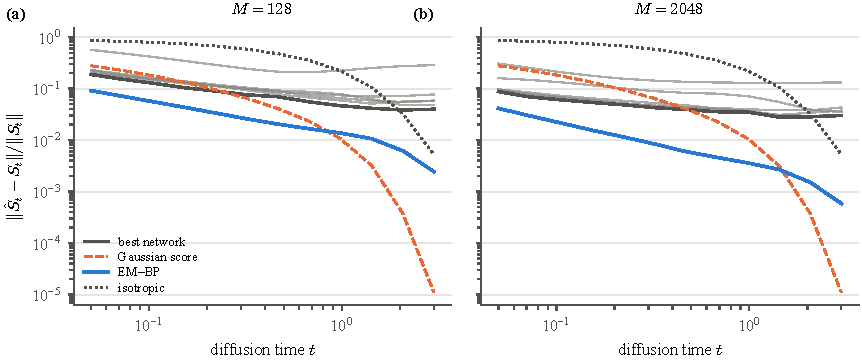
\includegraphics[width=\textwidth]{ff-nongaussian-gain.pdf}
  \caption{\textbf{Where the gain is.} Per-level relative score error against the exact score on the
  linear chain with Laplace noise, for $\nseq=128$ (a) and $\nseq=2048$ (b) training sequences: EM--BP
  (blue), the best of the six networks (thick grey; the other five thin), the Gaussian
  score (dashed) and the isotropic score (dotted). EM--BP is the best estimator at the lowest
  $\lvlFirstLevelsA$ (a) and $\lvlFirstLevelsB$ (b) of twelve levels. The Gaussian score, which is given the true
  covariance, overtakes it from $t=\lvlCrossA$ (a) and $t=\lvlCrossB$ (b) upward (the first level at which it is better,
  median over seeds), because nothing non-Gaussian is left to recover; no network is first at any level.}
  \label{fig:gain}
\end{figure*}

\begin{figure*}[t]
  \centering
  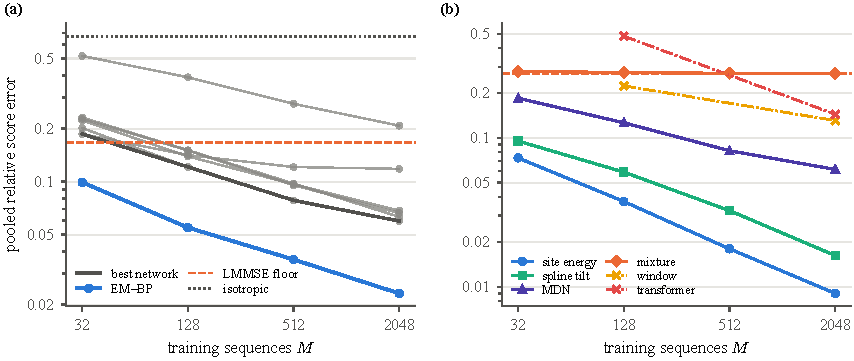
\includegraphics[width=\textwidth]{ff-sample-efficiency.pdf}
  \caption{\textbf{Sample efficiency.} Pooled relative score error against the number of training
  sequences. (a)~The linear chain with Laplace noise: EM--BP ($\ncomp=8$), the six networks (best in dark
  grey) and the LMMSE floor (dashed). (b)~The $\phi^4$ field at $\Temp=0.3$, $\latt=1$: the site energy, a
  spline-tilted kernel, an MDN kernel, the paper's mixture kernel and two networks, against the field's
  linear floor (dashed).}
  \label{fig:efficiency}
\end{figure*}

\paragraph{Generation.}
%% Included by 05-experiments.tex only when sections/generation-numbers.tex exists (E05 done).
Samples are drawn by the same reverse SDE (\genSteps{} steps on a geometric grid, one
Brownian path shared by every arm, \genSeeds{} seeds) from the exact score, the fitted
kernel, the LMMSE twin and the isotropic score, and compared with a reference sample of
the true law at $t_{\min}$ (\cref{tab:generation}). The exact arm's log-likelihood gap,
$\genLoglikgapDExact$ nats per sequence at $\nseq=2048$, is the sampler's own discretisation
error, the reference against which the other arms are read; the fitted kernel sits at $\genLoglikgapDEm$, the LMMSE twin at
$\genLoglikgapDLmmse$ and the isotropic score at $\genLoglikgapDIso$. The excess kurtosis of the
generated sequences' autoregressive residuals at $t_{\min}$, where the residual noise
lowers even the true law's value below the innovation's $3$, is $\genKurtgenDEm$ for the
fitted kernel against $\genKurtrefD$ for the true law and $\genKurtgenDLmmse$ for the twin, which by
construction generates Gaussian innovations: what the second-order estimator discards in
score error it discards in the samples.

Because the kernel is known after learning, generation does not need the reverse process at all: one
forward sweep from the learned kernel draws a sequence, and with the true kernel it samples at the Monte
Carlo floor of exact draws while costing $\genAncestralCostRatio\times$ less than a $200$-step reverse SDE
(\cref{app:tables}). A Gaussian score generates Gaussian sequences, whatever its accuracy at second order.


\section{Related work}
\label{sec:related}

\needsdata{Rewritten from docs/RELATED\_WORK\_SWEEP.md once the sweep is verified.}
Diffusion and score matching are due to \citet{sohl2015deep,ho2020denoising,song2021scorebased} and
\citet{hyvarinen2005estimation,vincent2011connection}; the score--posterior-mean identity is Tweedie's
\citep{robbins1956empirical,efron2011tweedie}. Solvable settings and the statistical mechanics of
diffusion \citep{biroli2023generative,biroli2024dynamical,cui2025solvable,raya2023spontaneous,ghio2024sampling} analyse memorisation and
speciation with targets that are Gaussian or mixture-like; hierarchical models supply
tractable non-Gaussian families \citep{sclocchi2025phase} on which U-Nets and transformers
implement belief propagation \citep{mei2024unets,garnierbrun2024transformers}. Our chain is the
degenerate tree of depth $\nsites$, and our estimator is classical: sum-product on a
chain is forward--backward \citep{baum1970,rabiner1989tutorial}, reducing to Kalman--RTS in the
Gaussian case; grid quadrature is Kitagawa's smoother \citep{kitagawa1987}; Fisher's
identity and EM are \citet{dempster1977maximum,cappe2005}. \Cref{thm:decay} belongs to the low-SNR literature. In Gaussian channels the
mutual information and the MMSE expand in the SNR with fourth-order statistics entering
at second order \citep{prelov2004second,guo2005mutual,dytso2023meta}; for latent-variable
models the log-likelihood expands with the order-$k$ term matching $k$-th moments
\citep{katsevich2023likelihood}, which gives the $\sigma^{2k}$ sample complexity of
multireference alignment and orbit recovery \citep{perry2019sample,bandeira2023estimation}
and, most closely, the layered Fisher-information geometry of \citet{balanov2026gmm}.
\citet{aarts2025cumulants} write the forward-process cumulant attenuation $e^{-nt}$ and
show that score networks regenerate the cumulants. \citet{wang2024gaussian} and
\citet{li2024hidden} observe that learned scores are dominated by their Gaussian part
over a wider noise range than a first-order bound suggests; \cref{eq:scoregap} is the
sharp rate behind that observation for a non-Gaussian chain, where the Gaussian part is
exactly the Kalman smoother. New here are the score-level statement with its constant
and crossover, the Markov (dependent) rather than i.i.d.\ latent structure, the exact
verification, and the learning consequences with an exact E-step rather than moment
matching.

\section{Conclusion}
\label{sec:conclusion}

For data that form a Markov chain, score estimation under diffusion noise reduces to posterior means, and a forward--backward sweep of
belief propagation computes them exactly for any continuous kernel, up to a quadrature we measure. The kernel itself is learnable from noised
sequences alone, by expectation--maximisation around the same sweep, so one can learn the local law and infer globally. The Gaussian kernel
is a clean check, since BP with Gaussian messages is the linear score and the Kalman smoother. On two chains whose scores are known, a linear chain with
non-Gaussian noise and the one-dimensional $\phi^4$ field, this estimator, with a kernel of a few parameters, beats the neural denoisers it is compared with
at every sample size, including at its own information interface; the kernel family is the real modelling choice, the five-parameter site energy being right for a
gradient flow and the paper's linear-drift mixture right for a linear chain and wrong for a double well; and a neural or unrestricted kernel earns its parameters only where
the simple family is misspecified.

The advantage is in data and understanding, not in wall-clock. Exact inference costs more per sequence than a network forward pass, by a factor that depends on the machine
and the grid, a coarser grid and a smaller kernel recover a large part of it for the field kernels, and a Fourier representation of the messages is not worth building. The
structure also has limits that can be computed: a latent shared by a whole sequence leaves a bias no sample size removes, which augmenting the state repairs; a kernel
outside the family leaves a floor the unrestricted kernel is built to detect; a coarse grid fails for narrow kernels. The comparison equalises the number of sequences under each
method's standard recipe and, separately, matches the information interface with no oracle on either side; it does not rank learning algorithms in general, and the networks
we time are the largest variants.

What the linear laboratory adds is a general fact about the channel: diffusion noise erases statistical structure order by order, at rates fixed by Hermite degree, so a score
learner that reaches only second order is bounded away from the truth by an $e^{-8t}$-scaled term whose content is the fourth-order moment. This explains where the structured
estimator gains and does not enter its exactness. Explicit structure recovers what the data still carry, and the price of the wrong structure is a bias that can be computed.


\section*{Impact statement}
This paper presents theoretical and empirical work on how diffusion noise erases
statistical structure and on learning structured dynamics from noised data, evaluated on
synthetic models with known ground truth. Its societal consequences are those of a better
understanding of generative diffusion models in general; we see no specific ethical
concern that requires discussion here.

\bibliography{references}
\bibliographystyle{icml2026}

\newpage
\appendix
\onecolumn
\section{Proofs}
\label{app:proofs}

\subsection{\Cref{prop:lmmse}}
Write $\lmsg^{\mathrm{p}}_i$ for the forward message at site $i$ after projection and
$\ell_i$ for the Gaussian unary likelihood. We show by induction that every projected
message equals the corresponding exact message of the covariance-matched Gaussian chain.
The initial message is Gaussian or projected to the Gaussian with the same first two
moments, which is the Gaussian chain's initial message. If $\lmsg^{\mathrm{p}}_{i-1}$ is
that chain's message, with mean $m$ and variance $v$, multiplying by $\ell_{i-1}$ gives
a Gaussian with the precision-weighted moments, identical in both chains; the transition
integral against $a_i=\corr a_{i-1}+\varepsilon_i$ is a convolution whose mean and
variance are $(\corr m,\corr^2v+\ivar)$ for every innovation with moments $(0,\ivar)$, so
$\Pgauss$ returns the Gaussian chain's next message. The backward sweep runs the same
argument with the inverted map $(m,v)\mapsto(m/\corr,(v+\ivar)/\corr^2)$, which is where
$\corr\neq0$ is used, starting from the terminal likelihood $\ell_{\nsites}$ (the flat
terminal message is not normalisable and contributes no factor). Every projected belief
is therefore the Gaussian chain's belief, whose posterior mean is linear in $\vx$ and
coincides with the LMMSE estimator $e^{-t}\Sig_0\Sig_t^{-1}\vx$. Since the recursion
never read $\innov$ beyond $(0,\ivar)$, the estimator is the same for every such law.
The algebraic steps (the two moment maps as integrals, the covariance identities, and
the optimality of the normal-equation gain in arbitrary dimension) are machine-checked
in Lean~4 (\codefile{lean/README.md}); the projection step itself is not.

\subsection{\Cref{thm:hermite}}
For $z\sim\normal{0}{1}$ and real $a$, $\alpha$ with $\beta=\sqrt{1-\alpha^2}$, the
generating function $e^{sx-s^2/2}=\sum_n\Hen{n}(x)s^n/n!$ evaluated at
$x=\alpha a+\beta z$ and averaged over $z$ gives
$e^{s\alpha a-s^2\alpha^2/2}=\sum_n\Hen{n}(a)(\alpha s)^n/n!$, hence
$\E_z\Hen{n}(\alpha a+\beta z)=\alpha^n\Hen{n}(a)$. The coordinates of $\vz$ are
independent given $\va$, so the product form holds for $H_\nu$; integrating over
$\va\sim\Pz$ requires only $\E|\va|^{|\nu|}<\infty$. The cases $n\le4$ are verified in
Lean as polynomial identities under the first four Gaussian moments.

\subsection{\Cref{thm:decay}}
\label{app:proof-decay}

\paragraph{Exact identities.}
With $\alpha=e^{-t}$ and $\Dt=1-\alpha^2$, Bayes' rule gives
$\Pt(\vx)=\gamma_{\Dt}(\vx)\,\E_{\Pz}\exp\bigl(\alpha\vx\cdot\va/\Dt-\alpha^2|\va|^2/2\Dt\bigr)$,
where $\gamma_{\Dt}$ is the $\normal{0}{\Dt\Id}$ density. Hence
$\log\Pt(\vx)=\log\gamma_{\Dt}(\vx)+\Lambda(s,b)$ with $s=\alpha\vx/\Dt$, $b=\alpha^2/\Dt$
and $\Lambda(s,b)=\log\E_{\Pz}\exp(s\cdot\va-b|\va|^2/2)$. For $b>0$ the tilted measure
is integrable for every $s$, so $\Lambda$ is real-analytic in $(s,b)$ on
$\Reals^{\nsites}\times(0,\infty)$, and its Taylor coefficients at the origin are the
joint cumulants of the linear form $s\cdot\va$ and the quadratic form $|\va|^2/2$;
$\E[\va\mid\vx]=\nabla_s\Lambda$ and $\score=-\vx/\Dt+(\alpha/\Dt)\nabla_s\Lambda$.

\paragraph{Grading.}
Expand $\Lambda$ in $(s,b)$ at the origin and grade a monomial $s^{j}b^{k}$ by $j+2k$;
since $s=O(\alpha)$ and $b=O(\alpha^2)$, the grade is the order in $\alpha$. By the
symmetry of $\Pz$ under $\va\mapsto-\va$ only even grades occur:
$\Lambda=\Lambda_2+\Lambda_4+R_6$, with
$\Lambda_2=\tfrac12s^{\!\top}\Sig_0s-\tfrac b2\operatorname{tr}\Sig_0$ and
\[
  \Lambda_4=\tfrac1{24}\kfour[s,s,s,s]
   -\tfrac b4\sum_i\operatorname{cum}(s\!\cdot\!\va,s\!\cdot\!\va,a_i,a_i)
   +\tfrac{b^2}8\sum_{ij}\operatorname{cum}(a_i,a_i,a_j,a_j),
\]
where $\operatorname{cum}$ is the joint cumulant under $\Pz$. Every fourth-order joint
cumulant of linear forms in $\va$ equals its value under the covariance twin plus a
linear contraction of $\kfour$, so $\Lambda_4-\Lambda_4^{\mathrm{G}}$ is linear in
$\kfour$ and $\Lambda_2=\Lambda_2^{\mathrm{G}}$. The remainder $R_6$ is the Taylor
remainder of grade six; on $\{|\alpha\vx|\le1\}$ it is bounded by
$C\alpha^6(1+|\vx|)^6$ with $C$ depending on the moments of $\Pz$ up to order eight.

\paragraph{Leading term of the score gap.}
$\score-\Sgauss=(\alpha/\Dt)\nabla_s(\Lambda-\Lambda^{\mathrm{G}})
=(\alpha/\Dt)\bigl[\nabla_s(\Lambda_4-\Lambda_4^{\mathrm{G}})+\nabla_sR_6-\nabla_sR_6^{\mathrm{G}}\bigr]$.
Substituting $s=\alpha\vx/\Dt$, $b=\alpha^2/\Dt$ and expanding in $\alpha$, the
grade-four term is
$\alpha^4\,\nabla_{\vx}\bigl[\tfrac1{24}\sum_{ijkl}\kfour[ijkl]\,{:}x_ix_jx_kx_l{:}\bigr]+O(\alpha^6(1+|\vx|)^5)$,
where ${:}\cdot{:}$ is the Wick (Hermite) product: the three contributions of $\Lambda_4$
combine into the Hermite form because $b=\alpha^2(1+O(\alpha^2))$ and the cumulant
contractions with $\delta_{ii}$ are exactly the terms that convert monomials into Hermite
polynomials. The $m$-th component is $\alpha^4\,\tfrac16\sum_{jkl}\kfour[mjkl]\,{:}x_jx_kx_l{:}$.

\paragraph{Second moment.}
Under $\gamma$, Wick's theorem gives
$\E_\gamma[{:}x_jx_kx_l{:}\,{:}x_{j'}x_{k'}x_{l'}{:}]$ equal to the number of perfect
matchings of $\{j,k,l\}$ with $\{j',k',l'\}$ respecting indices; contracted with the
symmetric tensor this yields
$\E_\gamma\bigl[(\tfrac16\sum_{jkl}\kfour[mjkl]{:}x_jx_kx_l{:})^2\bigr]
=\tfrac{3!}{36}\sum_{jkl}\kfour[mjkl]^2$, and summing over $m$,
$\E_\gamma\lVert\text{leading term}\rVert^2=\tfrac16\Frob{\kfour}^2\alpha^8$. Replacing
$\E_\gamma$ by $\E_{\Pt}$ costs a factor $1+O(\alpha^2\lmax)$: on the bulk,
$\Pt/\gamma=1+\alpha^2\tfrac12\langle\Sig_0-\Id,{:}\vx\vx^{\!\top}{:}\rangle+O(\alpha^4\lmax^2(1+|\vx|)^4)$,
and the degree-2 correction has zero $\gamma$-mean against the square of a degree-3
polynomial up to terms of relative size $\alpha^2\lmax$. The cross term between the
leading term and the grade-six remainder is $O(\alpha^{10}\lmax)$ by Cauchy--Schwarz and
the moment bound.

\paragraph{Tail.}
On $\{|\alpha\vx|>1\}$ the expansion is not used. There $|\score-\Sgauss|\le
2|\vx|/\Dt+\alpha(\E[|\va|\,|\vx]+|\E^{\mathrm G}[\va|\vx]|)/\Dt\le C(1+|\vx|)/\Dt$
because the tilted mean is bounded by a polynomial in $|\vx|$ under the moment
condition, while $\Pt(|\alpha\vx|>1)\le\exp(-c/\alpha^2)$ since $\vx_t$ is a Gaussian
convolution with variance at most one per coordinate. The tail contribution is therefore
$O(\exp(-c'e^{2t}))$, below every power of $\alpha$. Together,
$\E_{\Pt}\lVert\score-\Sgauss\rVert^2=\tfrac16\Frob{\kfour}^2e^{-8t}(1+O(e^{-2t}\lmax))$,
which is \cref{eq:scoregap}.

\paragraph{Information.}
$\partial_\theta\log\Pt=\partial_\theta\Lambda$. If $\partial_\theta\Sig_0\neq0$ the
grade-two term $\tfrac{\alpha^2}2\langle\partial_\theta\Sig_0,{:}\vx\vx^{\!\top}{:}\rangle$
leads, and $\E_\gamma$ of its square is
$\tfrac{\alpha^4}4\cdot2\Frob{\partial_\theta\Sig_0}^2$ by Wick, giving \cref{eq:info2}.
If $\partial_\theta\Sig_0=0$ the grade-four term
$\tfrac{\alpha^4}{24}\sum\partial_\theta\kfour[ijkl]{:}x_ix_jx_kx_l{:}$ leads, with
$\gamma$-second moment $\tfrac{4!}{24^2}\Frob{\partial_\theta\kfour}^2\alpha^8$, giving
\cref{eq:info4}; the corrections and the tail are handled as above. Since
${:}\vx\vx^{\!\top}{:}$ and the degree-four Hermite polynomials are $\gamma$-orthogonal,
the leading cross-information between a degree-2 and a degree-4 coordinate vanishes, so
the leading term of the efficient information of the degree-4 coordinate equals that of
its raw information. For the Gaussian chain $\vx_t\sim\normal{0}{\Sig_t(\theta)}$ exactly
and the stated trace formula is the Gaussian Fisher information; its limit
$e^{4t}I_t\to\tfrac12\Frob{\partial_\theta\Sig_0}^2$ follows from $\Sig_t\to\Id$ and
$\partial_\theta\Sig_t=\alpha^2\partial_\theta\Sig_0$, and is machine-checked in Lean
(\codefile{lean/README.md}, target~3).

\paragraph{The crossover.}
The expansion of $\Pt/\gamma$ used above is an expansion in $\alpha^2\Sig_0$, i.e.\ in
$\alpha^2\lmax(\Sig_0)$ in operator norm; for the chain $\lmax\le(1+\corr)/(1-\corr)$ by
the Toeplitz bound $\lmax\le\sum_k\corr^{|k|}$. This is the source of the factor
$\lmax$ in every remainder and of $\tstar=\tfrac12\log\lmax$; for the Gaussian chain the
exact formula shows the same scale directly, since $\Sig_t^{-1}$ is within
$\alpha^2\lmax$ of $\Id$ in operator norm.

\section{Numerical representation and its control}
\label{app:numerics}
\paragraph{The recursion.}
The two message sweeps of \cref{sec:setup} are
\begin{equation}
\begin{aligned}
  \lmsg_i(a)&\propto\!\int\!\kernel(a\mid a')\,\like(x_{i-1}\mid a')\,\lmsg_{i-1}(a')\dd a',\\
  \rmsg_i(a)&\propto\!\int\!\kernel(a''\mid a)\,\like(x_{i+1}\mid a'')\,\rmsg_{i+1}(a'')\dd a'',
\end{aligned}
\label{eq:bp}
\end{equation}
with $\lmsg_1\equiv\mu$, the initial law, and $\rmsg_{\nsites}\equiv1$; the site marginal is $\propto\lmsg_i\like\rmsg_i$
and Tweedie's identity turns its mean into the score.



Messages are represented on a uniform grid of $\ngrid$ points on
$[-\halfwidth,\halfwidth]$ with composite trapezoidal weights; the recursion is a scaled
linear-domain forward--backward whose discarded constants are accumulated so the
evidence $\log\Pt(\vx)$ of the discretised model is exact to floating point. Three
levels of exactness are kept apart: sum-product is exact at the level of functional
messages; forward--backward is exact for the discretised factor model; and that model
approximates the continuous chain with truncation (mass outside $[-\halfwidth,\halfwidth]$)
and quadrature (second order in the spacing) errors that are measured, not assumed.

\paragraph{Validation where the answer is known.}
\begin{proposition}[The Gaussian chain: score, smoother and sum-product coincide]
\label{prop:kalman}
Let the driving noise of \cref{eq:prior} be Gaussian, so that $\va\sim\normal{0}{\Sig_0}$ with
$(\Sig_0)_{ij}=\corr^{|i-j|}$, and let $\vx$ follow \cref{eq:channel}. Then
(i) $\score(\vx,t)=-\Sig_t^{-1}\vx$ and $\pmean{\va}=e^{-t}\Sig_0\Sig_t^{-1}\vx$, with
$\Sig_t=e^{-2t}\Sig_0+\Dt\Id$, and Tweedie's identity holds between them; (ii) every message of
\cref{eq:bp} is Gaussian, $\lmsg_i$ is the Kalman filter's prediction density
$p(a_i\mid x_{1:i-1})$ and $\lmsg_i\like$ its filtering density, and the site marginals
$\propto\lmsg_i\like\rmsg_i$ are those of the Rauch--Tung--Striebel smoother, whose means are
therefore $\pmean{\va}$ of (i).
\end{proposition}
The proof is in \cref{app:proofs}; \cref{fig:gaussian} measures it (\textsc{e39}). An RTS
smoother written without the BP code (\codefile{src/markov\_score/kalman.py}) agrees with the
closed form to $\gsRtsWorst$, and grid BP at the operating grid agrees with both to $\gsOpWorst$
at every one of the $\gsLevels$ levels. Refining the grid converges faster than any power of the
spacing, as the trapezoid rule does on Gaussian integrands, and reaches $10^{-10}$ by
$\ngrid=\gsNeedTmin$ at the smallest level, where the likelihood is narrowest, and by
$\ngrid=\gsNeedTmax$ at the largest; widening the domain at the operating spacing removes the
truncation error, which is $\gsAthreeTmin$ at $\halfwidth=3$. On the same grid the
moment-projected recursion of \cref{prop:lmmse} is off by up to $\gsProjWorst$: its backward
messages are Gaussians whose variance grows like $e^{2t}$, and the grid truncates them at
$\pm\halfwidth$. The proposition concerns functional messages, and the LMMSE floors reported
here are computed in closed form. Grid BP also reproduces brute-force enumeration of the
discretised posterior on short chains to double precision
(\codefile{tests/test\_gaussian\_bp\_equivalence.py},
\codefile{tests/test\_fisher\_bruteforce.py}).

\begin{figure}[t]
  \centering
  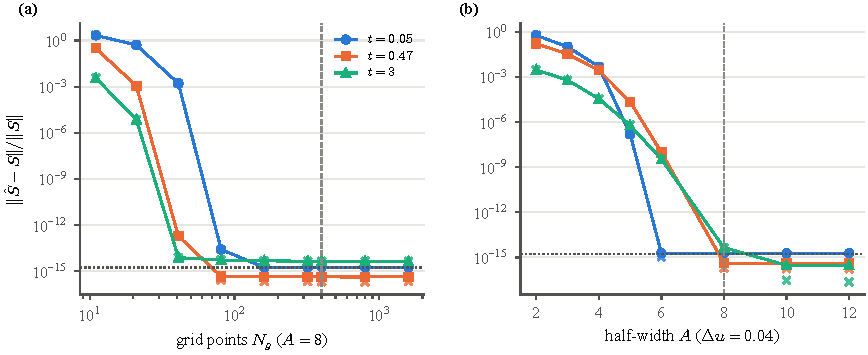
\includegraphics[width=\textwidth]{fig_gaussian_sanity.pdf}
  \caption{\textbf{The Gaussian sanity check (\textsc{e39}).} Pooled relative score error of
  grid BP against the closed-form score (lines) and against an independent
  Kalman--Rauch--Tung--Striebel smoother (crosses) on the Gaussian chain, at the smallest, a
  middle and the largest level. (a) Refining the grid at $\halfwidth=8$; (b) widening the domain
  at the operating spacing. Dashed: the operating grid. Dotted: the smoother against the closed
  form.}
  \label{fig:gaussian}
\end{figure}

Against a finer reference
($\ngrid=1601$, $\halfwidth=12$) the worst relative score error over the twelve levels
and four driving-noise families on ordinary draws is $\gcworstord$; under a
three-standard-deviation displacement the heavy-tailed families lose two orders
(\gcworstshift). The worst forward-message boundary occupancy is $\gcfwdedge$ and the
worst belief edge occupancy $\gcbeledge$ over $\gccells$ production cells.

\paragraph{The envelope, measured rather than inherited.}
\IfFileExists{sections/grid-envelope.tex}{%% Included by A2-numerics.tex only when sections/grid-envelope.tex exists (E11 done).
The validation above fixes the grid at the frozen configuration. Every other
configuration this paper touches---the other driving-noise families, the correlations of
the family ladder, the longer chains of the length study---inherits it, so we measured
it instead: $\gridFamilies$ driving-noise families $\times$ $\gridRhos$ correlations
$\times$ twelve levels $\times$ $\gridSeeds$ seeds, seven candidate grids against a
reference at $\ngrid=\gridRefN$, $\halfwidth=\gridRefA$.

At the frozen configuration the operating grid is comfortable: the pooled drift of the
posterior-mean field is $\gridFrozenDrift$, the worst single level $\gridFrozenDriftWorstLevel$,
and $\gridFrozenBoundary$ of the belief mass lies in the outermost $2\%$ of the domain.
Nothing reported at that configuration is in question.

Over the whole sweep the picture is different, and the difference is instructive: at
half-width $\gridHalfWidth$ the worst-case drift is \emph{flat} in the number of grid
points, $\gridFlatLo$ at $\ngrid=\gridFlatNlo$ and $\gridFlatHi$ at
$\ngrid=\gridFlatNhi$, and falls only when the domain widens---$\gridWiderADrift$ at
$(\gridWiderAN,\gridWiderAA)$ and $\gridWiderBDrift$ at $(\gridWiderBN,\gridWiderBA)$.
That is the signature of truncation rather than of quadrature, and it means refinement
in $\ngrid$ alone, which is what refinement has meant in this literature, cannot fix it.
The binding cell is the $\gridWorstFamily$ family at $\corr=\gridWorstRho$, and the
mechanism is a handful of sites: among the $8192$ sites of each seed's bundle,
$\audExceedCounts$ lie beyond $|a|=\gridHalfWidth$ (the analytic expectation is
$\audExceedExpected$), the largest at $|a|=\audExceedMax$. A site beyond the domain has
its posterior pinned to the boundary on every grid, which is the ``belief mass
$\gridWorstBoundary$ in the outer $2\%$'' of the diagnostic, and at the lowest level its
score error alone is the drift of $\gridWorstDrift$. For a polynomial tail the
expected exceedance count is Poisson with mean $\nseq\nsites\,P(|a|>\halfwidth)$, which no
finite domain makes zero: $\audExceedExpectedTwelve$ per $8192$ sites at
$\halfwidth=12$, $\audExceedExpectedSixteen$ at $\halfwidth=16$. Per replicate of the
family ladder of \cref{app:phase} ($\excChains$ chains of $\excSites$ sites) the same
expectation is $\excStudentRhozeroAeight$ sites at $\halfwidth=8$,
$\excStudentRhozeroAtwelve$ at $12$ and $\excStudentRhozeroAsixteen$ at $16$ for the
Student-$t_5$ chain at $\corr=0$, and below $\excLaplaceRhozeroAeight$ for every other
family and correlation; that ladder therefore quotes the heavy-tailed family from a
recomputation on the $(\phaseWideN,\phaseWideA)$ domain, where its pooled floor has
stopped moving (\textsc{e07b}, \textsc{e07c}); no claim in the body rests on it. The same
consideration governs the closure panel of \cref{fig:theory}: beyond $t\approx3$ the
reference on the $(801,8)$ grid carries the tail of the \emph{truncated} prior, and the
heavy-tailed families depart from the constant for that reason alone; on
$(3201,32)$ they reach it (\cref{app:audit}).

The envelope also has to cover the longer chains of the length study and of the regime
comparison, and it does (\textsc{e11b}: the same sweep at $\nsites\in\{\gridLenList\}$,
$\gridLenSeeds$ seeds). On the operating grid the worst pooled drift over the sweep is
$\gridLenWorstDriftThirtytwo$ at $\nsites=32$, $\gridLenWorstDriftSixtyfour$ at $64$ and
$\gridLenWorstDriftOnetwentyeight$ at $128$, a factor of at most $\gridLenWorstRatioMax$,
and at the frozen configuration $\gridLenFrozenDriftThirtytwo$, $\gridLenFrozenDriftSixtyfour$
and $\gridLenFrozenDriftOnetwentyeight$: the per-site quadrature error does not compound along
the chain, because the messages are renormalised at every site.

A second observation from the same sweep cuts the other way. The column-mass defect of
the discretised kernel, $\max_j|\sum_k \kernel(\gridpt{k}\mid \gridpt{j})w_k-1|$, grows
with correlation, from $\gridColMassLo$ at $\corr=\gridColMassLoRho$ to $\gridColMassHi$
at $\corr=\gridColMassHiRho$, and the reason is again the domain and not the spacing: the
maximum sits in the outermost columns, where a kernel centred at $\corr\gridpt{j}$ with
$|\gridpt{j}|$ near $\halfwidth$ loses the part of its mass beyond the domain, so the
defect is flat in $\ngrid$, falls as the domain widens, and is at machine precision in the
interior columns at every $\corr$. It is not predictive of the error: at
$\corr=\gridColMassHiRho$ the drift is $\gridColMassDriftHiRho$, because the recursion
renormalises every message and the affected columns carry almost no belief. We report it
as a diagnostic and not as an error bar. The uniform family is the one exception to the
quadrature picture: its kernel is discontinuous, the trapezoidal rule is first-order on
it, and its worst-level drift is largest on the coarsest spacing rather than the
narrowest domain.
}{\needsdata{E11 pending: the quadrature envelope across families, correlations and levels}}

\paragraph{Refinement on the reported estimands.}
\IfFileExists{sections/refinement-numbers.tex}{%% Included by A2-numerics.tex only when sections/refinement-numbers.tex exists (E04 done).
Re-scoring the validation-selected kernels of the capacity experiment on their own test
bundles at $\ngrid=801$ and $1601$ ($\halfwidth=8$) and at $\halfwidth=10$
($\ngrid=801$), with the reference recomputed at each resolution, moves the pooled error
of EM--BP ($\ncomp=8$) by at most $\refMoveEmeightDfine\%$, $\refMoveEmeightDfinest\%$
and $\refMoveEmeightDwide\%$ at $\nseq=2048$ (maximum over $\refSeeds$ seeds), and the
LMMSE floor by at most $\refMoveLmmseDfine\%$; the reference score itself moves by
$\refRefMoveDfine\%$ between $\ngrid=401$ and $801$. The reported effects are three
orders of magnitude larger than the discretisation.
}{\needsdata{E04 pending: movement of the headline cells under refinement}}

\paragraph{Floors in the theory verification.}
The outer-product information estimate of a shape coordinate is a small residual of
order-one quantities; for the kinked Laplace density its quadrature floor is reached
near $t=2.5$ at $\ngrid=801$ (the replicate spread stops shrinking), which is why
\cref{fig:theory}b reports the asymptotic slope on the smooth members of the family. The
closure gap of the uniform family reaches the double-precision floor of the BP means
near $t=3.5$, where its squared gap is $10^{-13}$ per chain.

\section{Experimental protocol and provenance}
\label{app:protocol}

\paragraph{Frozen configuration.}
Laplace chain unless stated, $\corr=0.85$, $\ivar=1-\corr^2$, $a_1\sim\normal{0}{1}$,
$\nsites=32$; grid $\ngrid=401$, $\halfwidth=8$; twelve log-spaced levels
$t\in[0.05,3.0]$; other families Gaussian, Student-$t$ ($\nu=5$), uniform, symmetric
two-component mixture ($\kappa=0.6$), generalised Gaussian ($\beta\in[1,6]$), all
variance-matched. Sixteen confirmatory seeds $0$--$15$; development seeds
$10000$--$10001$ for every architecture and hyperparameter choice (one $16{,}000$-step
run per configuration at $\nseq\in\{32,2048\}$, ranked by pooled bulk risk). Validation and test
bundles are drawn per seed ($1024$ and $2048$ sequences) from streams disjoint from
every training stream; their hashes are stored with every row so pairing across arms is
checkable.

\paragraph{Estimand.}
Schedule-pooled relative score error
$\bigl(\sum_t\sum_{j,i}(\hat s_t(\vx_j)_i-s_t(\vx_j)_i)^2/\sum_t\sum_{j,i}s_t(\vx_j)_i^2\bigr)^{1/2}$
on all sites (the headline), on the interior sites $5$--$28$ (used for selection), and on
the centre site (diagnostic). Ratios are formed within seed and averaged; intervals are
percentile bootstraps over seeds.

\paragraph{Arms.}
EM--BP: mixture-innovation kernel, $\ncomp$ as stated, $\corr$ initialised at $0.3$, one
noised view per sequence with sequences split evenly across the twelve levels, checkpoint
ladder $\{10,20,40,60,80,120,160,220,300,400\}$ selected on the validation bundle.
Networks: trained by denoising score matching on the clean sequences with the level and
the corruption redrawn at every step, batch $64$, Adam, gradient clipping at $1$, both
output parameterisations, checkpoint ladder to $32{,}000$ steps selected on the validation
bundle; the information-matched arm trains by implicit score matching on the same
one-view noisy bundle as EM--BP and selects on the implicit objective of a held-out noisy
bundle.

\paragraph{Provenance.}
Every run directory carries the commit, the dirty-tree list on the code path, the
resolved configuration digest, the seeds, host and environment; a generator refuses to
emit a table from a run whose code path was dirty, from an incomplete design, or from
cells whose narrowest fitted component is under two grid cells. Every number in this
paper is a macro emitted by such a generator; the manuscript check
(\codefile{tools/check\_manuscript.py}) fails the build on any typed decimal.

\section{The oracle ladder}
\label{app:oracles}

\begin{table}[h]
\centering
\caption{Schedule-pooled relative score error of the two oracles against the tree-exact
reference, 512 chains per family at the frozen configuration. The LMMSE column is the
floor of every second-order estimator (\cref{prop:lmmse}).}
\begin{tabular}{lccc}
\toprule
family & excess kurtosis & isotropic $-\vx$ & LMMSE, true $\Sig_0$ \\
\midrule
Laplace & $+3$ & \isoFloorLaplace & \lmmseFloorLaplace \\
Student-$t_5$ & $+6$ & \isoFloorStudent & \lmmseFloorStudent \\
uniform & $-1.2$ & \isoFloorUniform & \lmmseFloorUniform \\
bimodal & $-0.72$ & \isoFloorBimodal & \lmmseFloorBimodal \\
Gaussian & $0$ & \isoFloorGaussian & \lmmseFloorGaussian \\
\bottomrule
\end{tabular}
\end{table}

\section{The second-order floor across correlation}
\label{app:phase}
The frozen configuration fixes $\corr=0.85$. The price of second-order closure is a function
of $\corr$ as well as of the innovation law, and this appendix reports it over
$\corr\in\{0,0.3,0.6,0.85,0.95\}$ for five families on the twelve-level schedule, computed
from the exact score with no estimation involved.
The heavy-tailed family is quoted from a recomputation on the
$(\phaseWideN,\phaseWideA)$ domain (\textsc{e07c}): on the operating grid the quadrature
sweep of \cref{app:numerics} places its $\corr=0$ cell outside the validated envelope, one
to two sites per bundle lying beyond the domain and pinned to its boundary. Widening the
domain moves its pooled floor by at most $\phaseStudentMoveOperating$ from $(801,8)$ to
$(801,12)$ and by at most $\phaseStudentMoveWide$ from $(801,12)$ to
$(\phaseWideN,\phaseWideA)$ (\textsc{e07b}, \textsc{e07c}), and every other family by at
most $\phaseOtherMoveWide$ between the operating and the widest grid; the other families
are quoted from the operating grid, where they are converged.
\IfFileExists{sections/phase-numbers.tex}{%% Included by 05-experiments.tex only when sections/phase-numbers.tex exists (E07 done).
\begin{figure}[t]
  \centering
  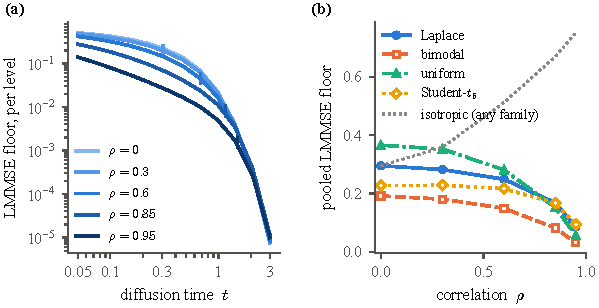
\includegraphics[width=\columnwidth]{fig_phase.pdf}
  \caption{\textbf{The second-order floor across correlation.} (a)~Per-level LMMSE
  floor on the Laplace chain for five $\corr$ (ticks: $\tstar(\corr)$); the floor
  collapses after the crossover. (b)~Schedule-pooled floor against $\corr$ for four
  innovation families, with the isotropic reference: strong correlation makes the score
  energy second-order-dominated, so the relative price of closure falls with $\corr$ while
  the absolute fourth-order structure does not.}
  \label{fig:phase}
\end{figure}
\paragraph{Across correlation.}
The floor is a function of the innovation law and of $\corr$ (\cref{fig:phase}): on the
Laplace chain it is $\phaseLmmseLaplaceRhozero$ for independent sites, $\phaseLmmseLaplaceRhozeropeightfive$
at the frozen $\corr=0.85$ and $\phaseLmmseLaplaceRhozeropninefive$ at $\corr=0.95$, where
$\tstar=\phaseTstarRhozeropninefive$ and the covariance carries most of the score energy
until late in the schedule. The families order by the size of their fourth cumulant at
every $\corr$; the isotropic reference rises with $\corr$ because the covariance itself is
what an unstructured estimator must learn first.
}{}

\section{Capacity: the previous reading, and why it is void}
\label{app:capacity}
An earlier study of this model compared innovation mixtures of $\ncomp\in\{1,2,4,8,16\}$
at $\nseq\in\{128,512\}$ over sixteen seeds and concluded that no capacity improved on a
single Gaussian innovation, attributing the estimator's margin over the networks to the
Markov factorisation and its covariance alone. That sweep is void for a reason prior to
any reading of it: its training draw re-created the random generator for every sequence,
so every arm at every capacity and seed was fitted to a single chain of $\nsites$ sites
(its validation and test bundles were drawn correctly). The signature is in its own
numbers: \cref{prop:lmmse} places a correctly fitted $\ncomp=1$ kernel on the LMMSE floor,
$\lmmseFloorLaplace$ on the Laplace chain, where \cref{sec:experiments} and all fifteen
cells of the regime sweep land to $\regIdentMax$, and the earlier sweep's single-Gaussian
arm scatters across a range several times wider. The stopping asymmetry that sweep also
shows (its likelihood tolerance fired for almost every single-Gaussian cell and for no
cell with $\ncomp\ge4$, so that the richer arms reported checkpoints far past their
optimum) is the behaviour of \textsc{em} on one chain, not evidence about capacity in
either direction; we had first read it as the explanation of the earlier conclusion, and
withdraw that reading. The capacity experiment of \cref{sec:experiments} draws every
chain independently, asserts it, and selects the checkpoint identically for every
capacity on a per-seed validation bundle; the same defect was found and fixed in one of
our own drivers before any of its numbers reached a page (\cref{app:protocol}).

\section{Capacity across the innovation family}
\label{app:family}
\IfFileExists{sections/family-numbers.tex}{%% Included by 05-experiments.tex only when sections/family-numbers.tex exists (E02b done).
\begin{figure}[t]
  \centering
  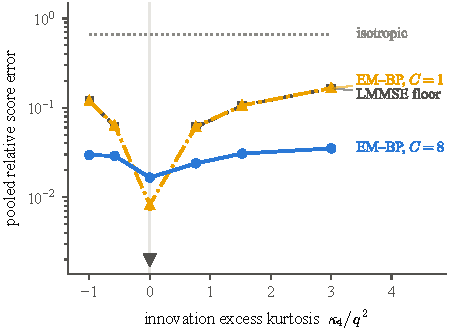
\includegraphics[width=\columnwidth]{fig_family.pdf}
  \caption{\textbf{Capacity buys exactly what the closure discards.} Pooled relative score
  error against the innovation's excess kurtosis for the generalised-Gaussian family at
  fixed $\corr$ and variance ($\nseq=\famSize$, $\famSeeds$ seeds, $\pm$ s.e.): the
  Gaussian-innovation kernel tracks the LMMSE floor, which is the exact price of
  second-order closure for each member; the mixture kernel tracks the exact score, and
  the two meet at the Gaussian member, where there is nothing beyond second order to
  learn.}
  \label{fig:family}
\end{figure}
Moving the innovation from Laplace (excess kurtosis $+3$) through the Gaussian to the
platykurtic end at fixed covariance (\cref{fig:family}), the LMMSE floor falls from
$\famLmmseBone$ to zero at $\beta=2$ and rises again to $\famLmmseBsix$; the
Gaussian-innovation kernel follows it, and the mixture kernel stays near
$\famEmeightBone$--$\famEmeightBsix$ throughout. The paired gain of $\ncomp=8$ over
$\ncomp=1$ is $\famDiffBone$ ($[\famDiffBonelo,\famDiffBonehi]$) at the Laplace end and
$\famDiffBtwo$ ($[\famDiffBtwolo,\famDiffBtwohi]$) at the Gaussian member, where the
two kernels are the same estimator up to sampling noise. Non-Gaussian capacity is worth
what \cref{thm:decay} says it is worth: the fourth-order structure the covariance twin
leaves behind.
}{\needsdata{E02b queued}}

\section{The capacity contrast across regimes}
\label{app:regimes}
\IfFileExists{sections/regime-numbers.tex}{%% Included by 05-experiments.tex only when sections/regime-numbers.tex exists (E13 done).
The capacity result above is measured at one point of the model's parameter space, so we
re-ran the contrast that carries it across $\regCells$ regimes: correlations from
$\regRhoLo$ to $\regRhoHi$ and chain lengths from $\regLenLo$ to $\regLenHi$, everything
else at the frozen protocol, $\regSeeds$ seeds each. The mixture beats the Gaussian
kernel in $\regAllExcludeZero$ cells with the paired interval excluding zero, by
$\regGainStrongest$ at the most favourable corner and $\regGainWeakest$ at the least.
The sweep also checks the apparatus at every point rather than only at the frozen
configuration: \cref{prop:lmmse} says the $\ncomp=1$ arm must coincide with the LMMSE of
the true covariance, and it does, to $\regIdentMax$ in the worst of the $\regCells$
cells, with a fitted excess kurtosis of at most $\regFitKurtOneMax$ in absolute value.
The $\ncomp=8$ arm recovers the innovation's true excess kurtosis of $3$ everywhere
($\regFitKurtLo$ to $\regFitKurtHi$ across correlations), and its spread widens from
$\pm\regFitKurtSdLo$ to $\pm\regFitKurtSdHi$ as $\corr$ rises---the shape becomes harder
to see, not differently placed.

The advantage itself shrinks monotonically with $\corr$, which is the direction
\cref{sec:theory} gives: a strongly correlated chain has a nearly Gaussian marginal, its
excess kurtosis falling as $3(1-\corr^2)/(1+\corr^2)$ from $\regKurtHi$ at
$\corr=\regRhoLo$ to $\regKurtLo$ at $\corr=\regRhoHi$, so there is less fourth-order
structure for capacity to buy. We report this as a direction and not as a rate: the
pooled error runs over a schedule whose informative window moves with $\corr$, so its
trend is not the exponent of \cref{thm:gap} and we do not fit one to it.
}{\needsdata{E13 pending}}

\section{Generation and length extrapolation: the tables}
\label{app:tables}
\IfFileExists{sections/generation-numbers.tex}{%% GENERATED by tools/make_generation_numbers.py from outputs/E05 -- do not hand-edit.
\begin{table}[t]\centering\small\setlength{\tabcolsep}{4pt}
\caption{Generated samples against the true law at $t_{\min}$: mean log-likelihood gap $\Delta\ell$ to the reference sample under the true $P_{t_{\min}}$ (exact evidence; the exact arm's gap is the sampler's discretisation floor), innovation excess kurtosis $\hat\kappa_4$, lag fourth cumulant, sliced $W_2$; the row marked \emph{reference} carries the reference sample's own statistics. Mean over seeds.}
\label{tab:generation}
\begin{tabular}{@{}llrrrr@{}}
\toprule
$\nseq$ & arm & $\Delta\ell$ & $\hat\kappa_4$ & lag-$\kappa_4$ & $W_2$ \\
\midrule
128 & \emph{reference} & -- & 1.94 & 0.000 & -- \\
 & exact & 0.074 & 1.86 & 0.000 & 0.051 \\
 & em--bp & 0.204 & 1.68 & 0.000 & 0.078 \\
 & lmmse & 1.761 & 0.00 & 0.000 & 0.053 \\
 & isotropic & 46.241 & 0.00 & 0.006 & 0.244 \\
 & net:bigru & 0.752 & 1.10 & 0.006 & 0.160 \\
 & net:window & 1.284 & 1.27 & 0.004 & 0.154 \\
\midrule
2048 & \emph{reference} & -- & 1.94 & 0.000 & -- \\
 & exact & 0.070 & 1.87 & 0.000 & 0.051 \\
 & em--bp & 0.164 & 1.80 & 0.001 & 0.055 \\
 & lmmse & 1.766 & 0.00 & 0.000 & 0.053 \\
 & isotropic & 46.295 & 0.00 & 0.010 & 0.244 \\
 & net:bigru & 0.385 & 1.55 & 0.003 & 0.167 \\
 & net:window & 1.115 & 1.46 & 0.003 & 0.139 \\
\bottomrule
\end{tabular}
\end{table}
}{}
\IfFileExists{sections/baseline-numbers.tex}{%% GENERATED by tools/make_baseline_numbers.py -- do not hand-edit.
\begin{table}[t]\centering\small\setlength{\tabcolsep}{4pt}
\caption{Length extrapolation at $\nseq=2048$: pooled relative score error of estimators fitted at $\nsites=32$ and evaluated against the tree-exact score of longer chains, mean over $\baseSeeds$ seeds. Longer chains are slightly easier (proportionally fewer boundary sites), so a length-agnostic arm should improve a little; the transformer instead breaks down beyond its training length.}
\label{tab:length}
\begin{tabular}{@{}lcccc@{}}
\toprule
arm & $\nsites=32$ & $\nsites=64$ & $\nsites=128$ & $\nsites=256$ \\
\midrule
bi-GRU & 0.060 & 0.057 & 0.057 & 0.056 \\
EM--BP & 0.023 & 0.023 & 0.023 & 0.023 \\
TCN & 0.068 & 0.066 & 0.065 & 0.064 \\
transf. & 0.063 & 0.243 & 0.514 & 0.703 \\
U-Net & 0.066 & 0.064 & 0.062 & 0.062 \\
window & 0.118 & 0.099 & 0.088 & 0.082 \\
\bottomrule
\end{tabular}
\end{table}
}{}


\end{document}
